\chapter{Simulation: Binomial Scenarios}
\section{Introduction}
This scenario models an enviroment where users have a fixed position in the space. There are some users which receive stronger signal from antenna, so they have an higher mean CQI, and others which are far from antenna and then they have smaller mean CQI. The requirements state that the distribution of CQIs must have a binomial distribution. To satisfy these, at each timeslot \(t_{j}\), every \texttt{Mobile Station} \(i\) generates a RV \(X_{i,t_{j}} \sim Bin(14,p_{i})\), and then \(CQI_{i,t_{j}} = X + 1\). By using this trick \(CQI_{i,t_{j}} \in \{1,15\}\) and it has a binomial distribution. In order to have different means we chose the following values for parameters \(p_{i}\).
\begin{lstlisting}[caption={omnet.ini - p parameters}]
	CellularNetwork.users[0].cqi_binomial_p = 0.13
	CellularNetwork.users[1].cqi_binomial_p = 0.22
	CellularNetwork.users[2].cqi_binomial_p = 0.31
	CellularNetwork.users[3].cqi_binomial_p = 0.40
	CellularNetwork.users[4].cqi_binomial_p = 0.49
	CellularNetwork.users[5].cqi_binomial_p = 0.58
	CellularNetwork.users[6].cqi_binomial_p = 0.67
	CellularNetwork.users[7].cqi_binomial_p = 0.76
	CellularNetwork.users[8].cqi_binomial_p = 0.85
	CellularNetwork.users[9].cqi_binomial_p = 0.94
\end{lstlisting}
As in the previous scenario we will analyze the performance about throughput and response time by using both schedulers. Before doing simulation we can do some conjectures. Note that in this scenario mean CQI are sensibly different so we expect that \(user[9]\), that has highest probability to generate high CQI, will have highest throughput. However the two different scheduler will influence the throughput and response time in different ways.
%Moreover we can suppose that it will take advantage of Best CQI policy and will get an higher throughput despite other users. Otherwise \(user[0]\), which has lower mean CQI, we can suppose it will decrease its throughput when it is used the Best CQI Scheduler.

These are the simulation parameters used in both binomial scenarios:
\begin{itemize}
	\item \(n=10\)
	\item \(packetsize_{i} \sim U(3,75), \quad 0 \le i \le n-1\)
	\item \(CQI_{i} \sim Bin(14,p_{i})+1, \quad 0 \le i \le n-1\)
	\item \( \lambda = \lambda_{i} = 0.1 + 0.5k, \quad k\in\{1,2\ldots,19\}, \quad 0 \le i \le n-1\)
\end{itemize}

\section{Binomial, Fair Scheduler}
In this scenario the scheduler is the basic Round Robin scheduler.

\begin{figure}[H]
  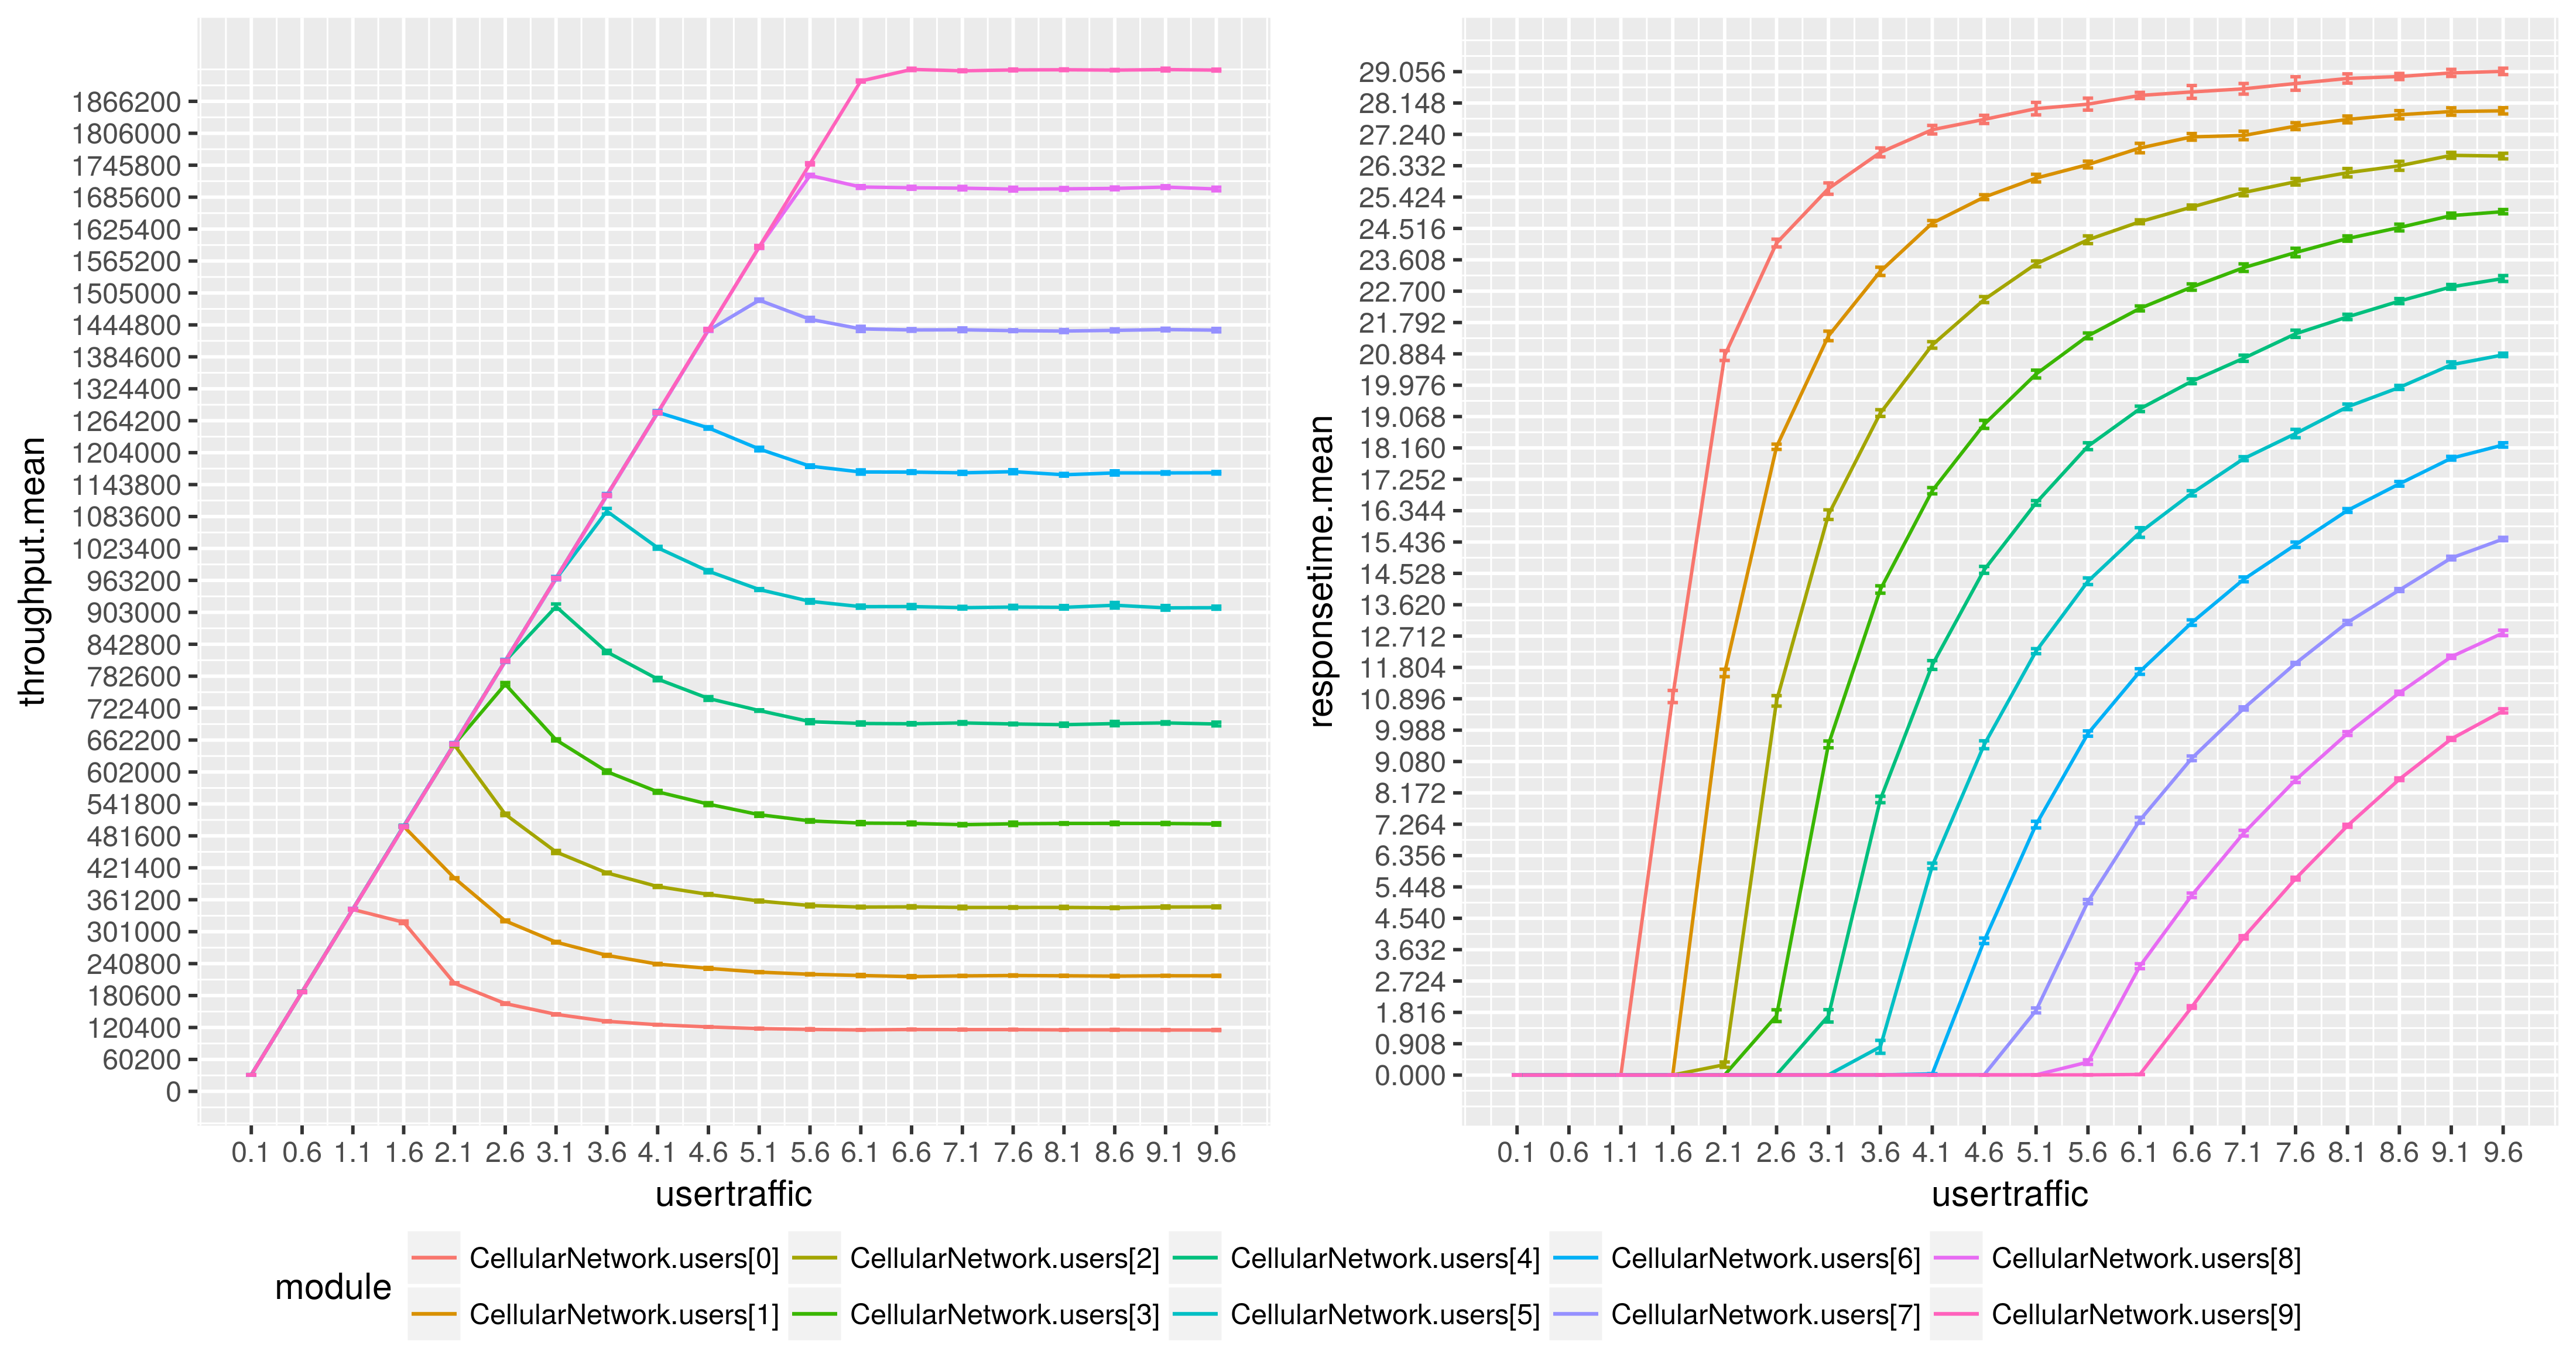
\includegraphics[width=1\textwidth]{images/all-binom}
  \caption{Binomial scenario - Fair: throughput, response time}
  \label{fig:Binomial scenario - Fair: throughput, response time}
\end{figure}
Users have very different throughput as we expected. When \( 0 < \lambda \leq 1\), all users have the same throughput because the traffic is very low and the resources provided by the frame are quite enough to satisfy all users. However this is a very special case, we can see that as \(\lambda\) increases users having lower mean CQIs saturate. The scheduler is always fair but users with higher mean CQIs have bigger RBs inside the frame that can carry more data. Saturation points follow the distribution of CQIs among users, so users with lower CQI, on average, saturate before, otherwise users with higher CQI exploit better the frame and saturate with higher \(\lambda\) rate. 
By analyzing the throughput plot we observe that users have a small peak near the saturation point and then their throughput decrease and approches to an horizontal line. The explaination is quite easy. If \(\lambda\) rate is \textit{small} users with higher mean CQI use few RBs to empty their queue, so the frame filling algorithm has free RBs to distribute among other users. When \(\lambda\) rate becomes \textit{high} also users with higher mean CQI require the lots of RBs and the effect of residual frame fill is limited. 

In the previous graph we observe that response time seems to approch to \(ST/2\). As explained in the chapter ~\ref{Validation-2} this strange behavior occurs when response time grows linear to infinity. In order to have a correct sight of what happen to response time we must zoom that plot.
\begin{figure}[H]
  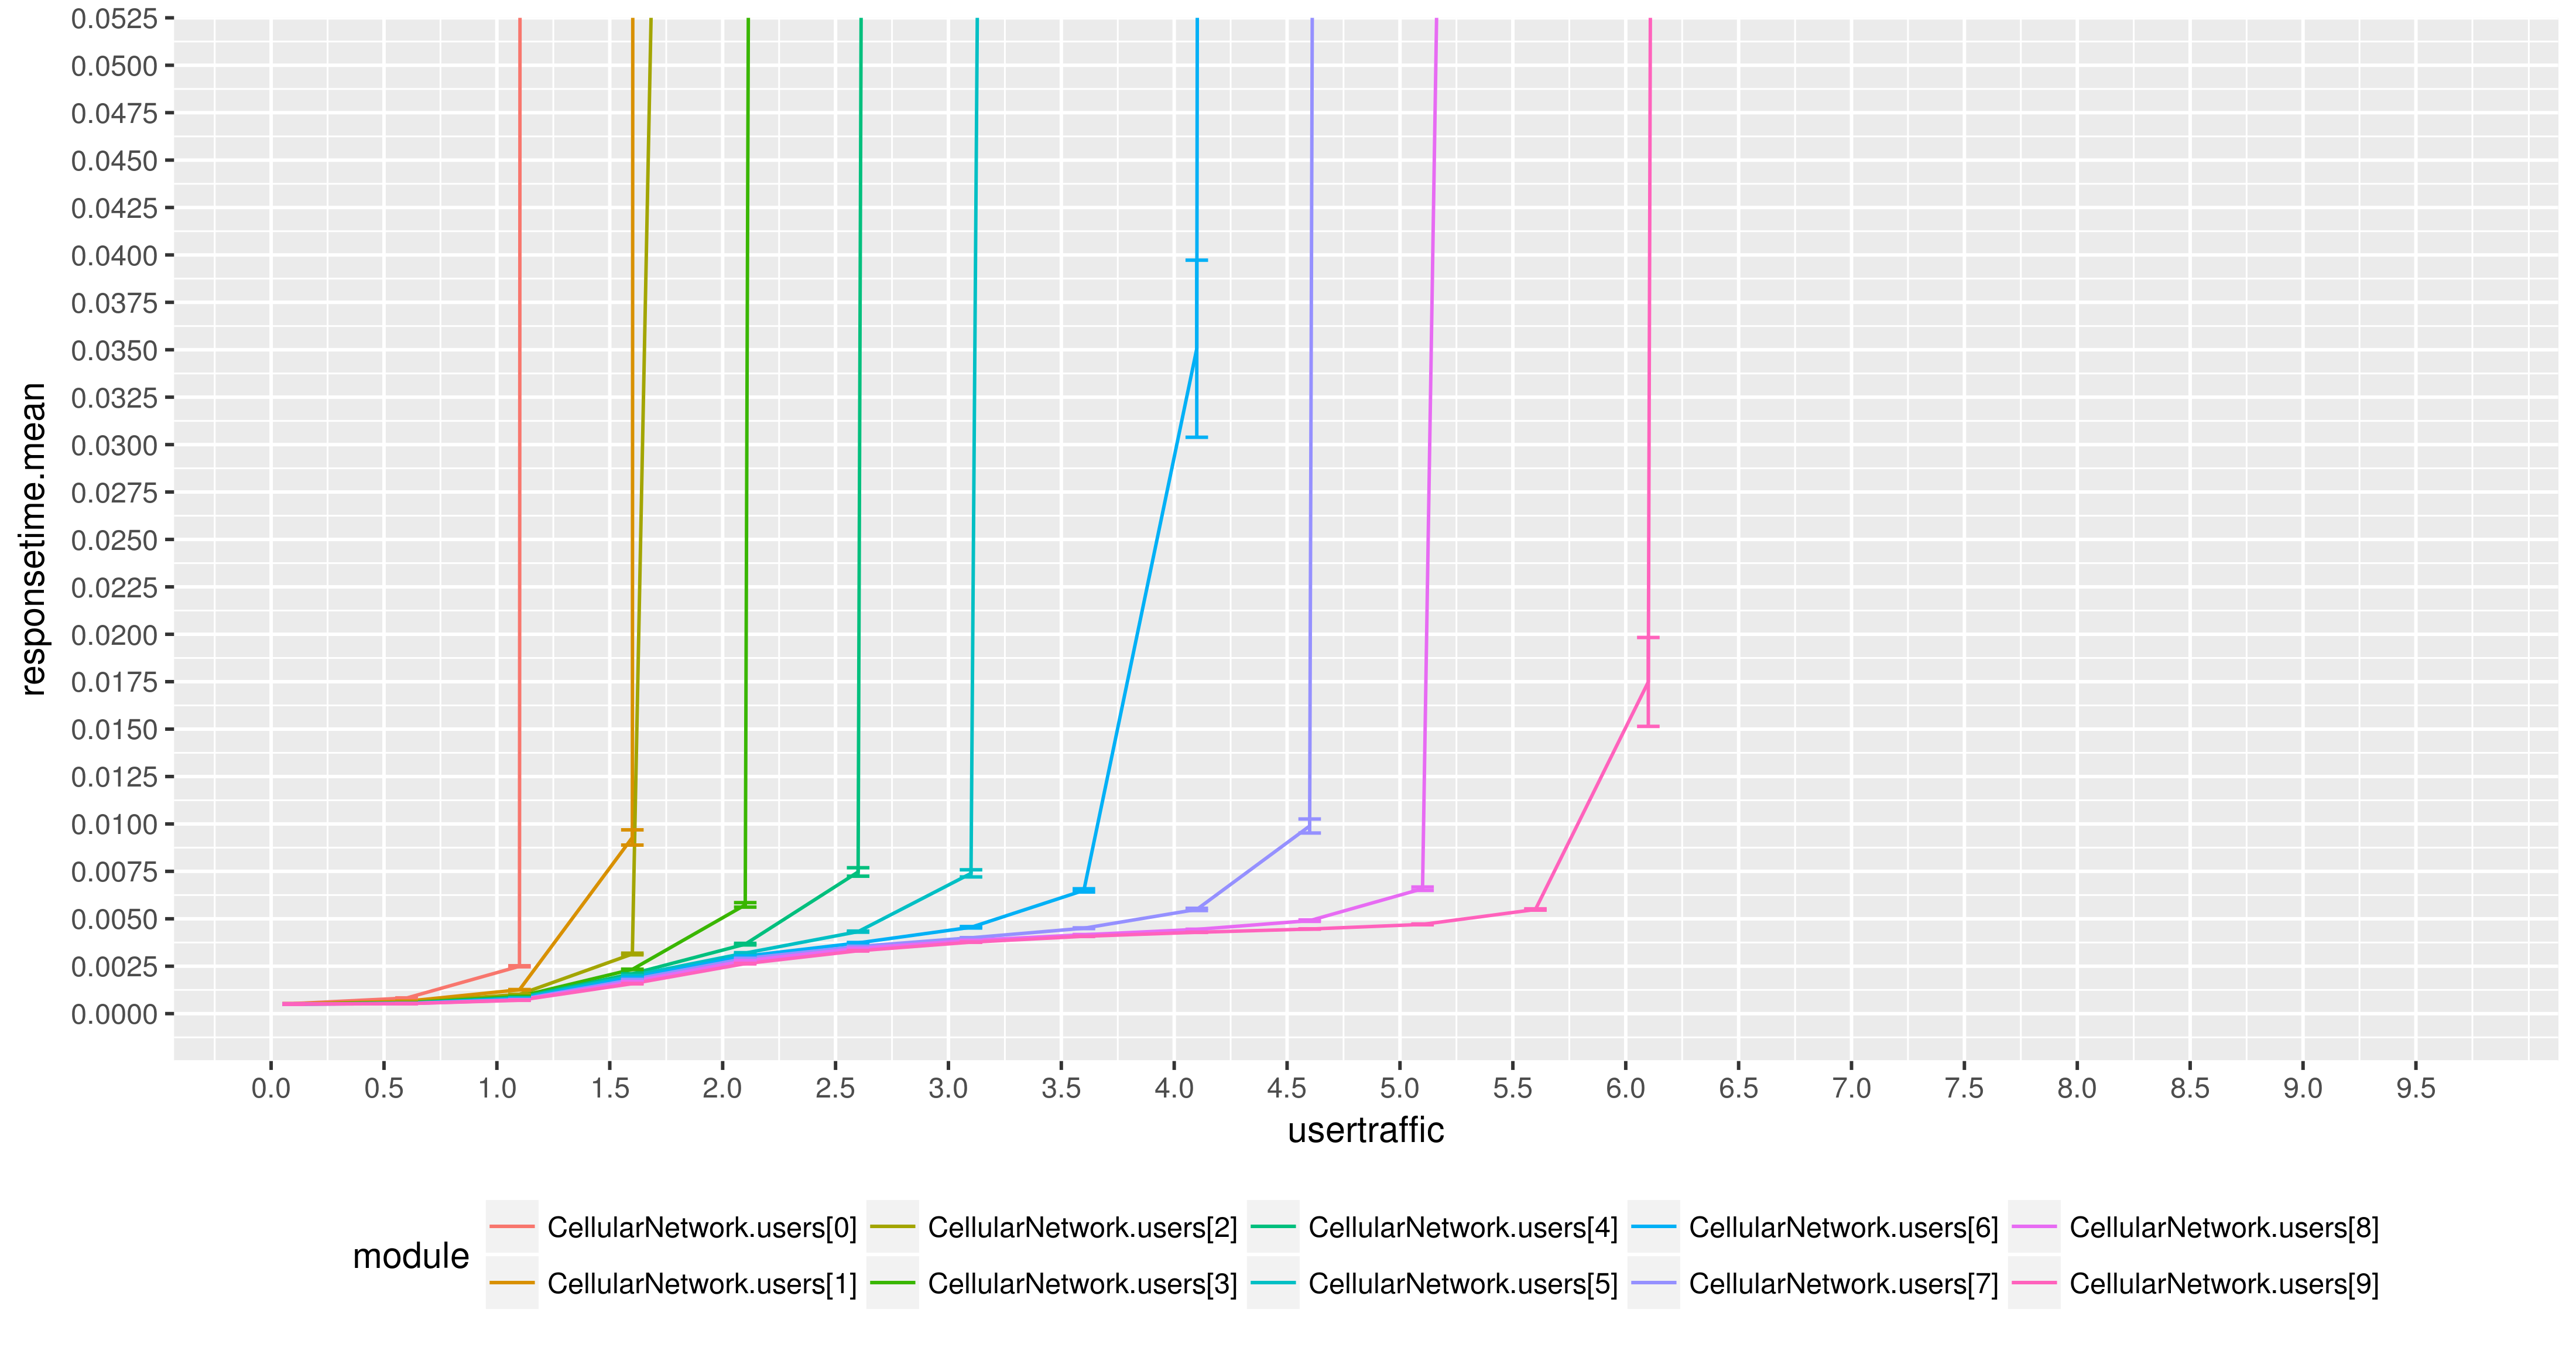
\includegraphics[width=1\textwidth]{images/allrt-binom}
  \caption{Binomial scenario - Fair: response time zoom}
  \label{fig:Binomial scenario - Fair: response time zoom}
\end{figure}

It is necessary to remark that the frame filling policy can have a strong impact on distribution of the throughput and response time. Let's consider, for example, a different policy: 
\begin{itemize}
\item The residual space in the frame is filled by considering all users \(j\), where \(j = (currentUser+1) \bmod n\) and so on, wrapping until user \((j-1) \bmod n\).
\end{itemize}
\begin{figure}[H]
  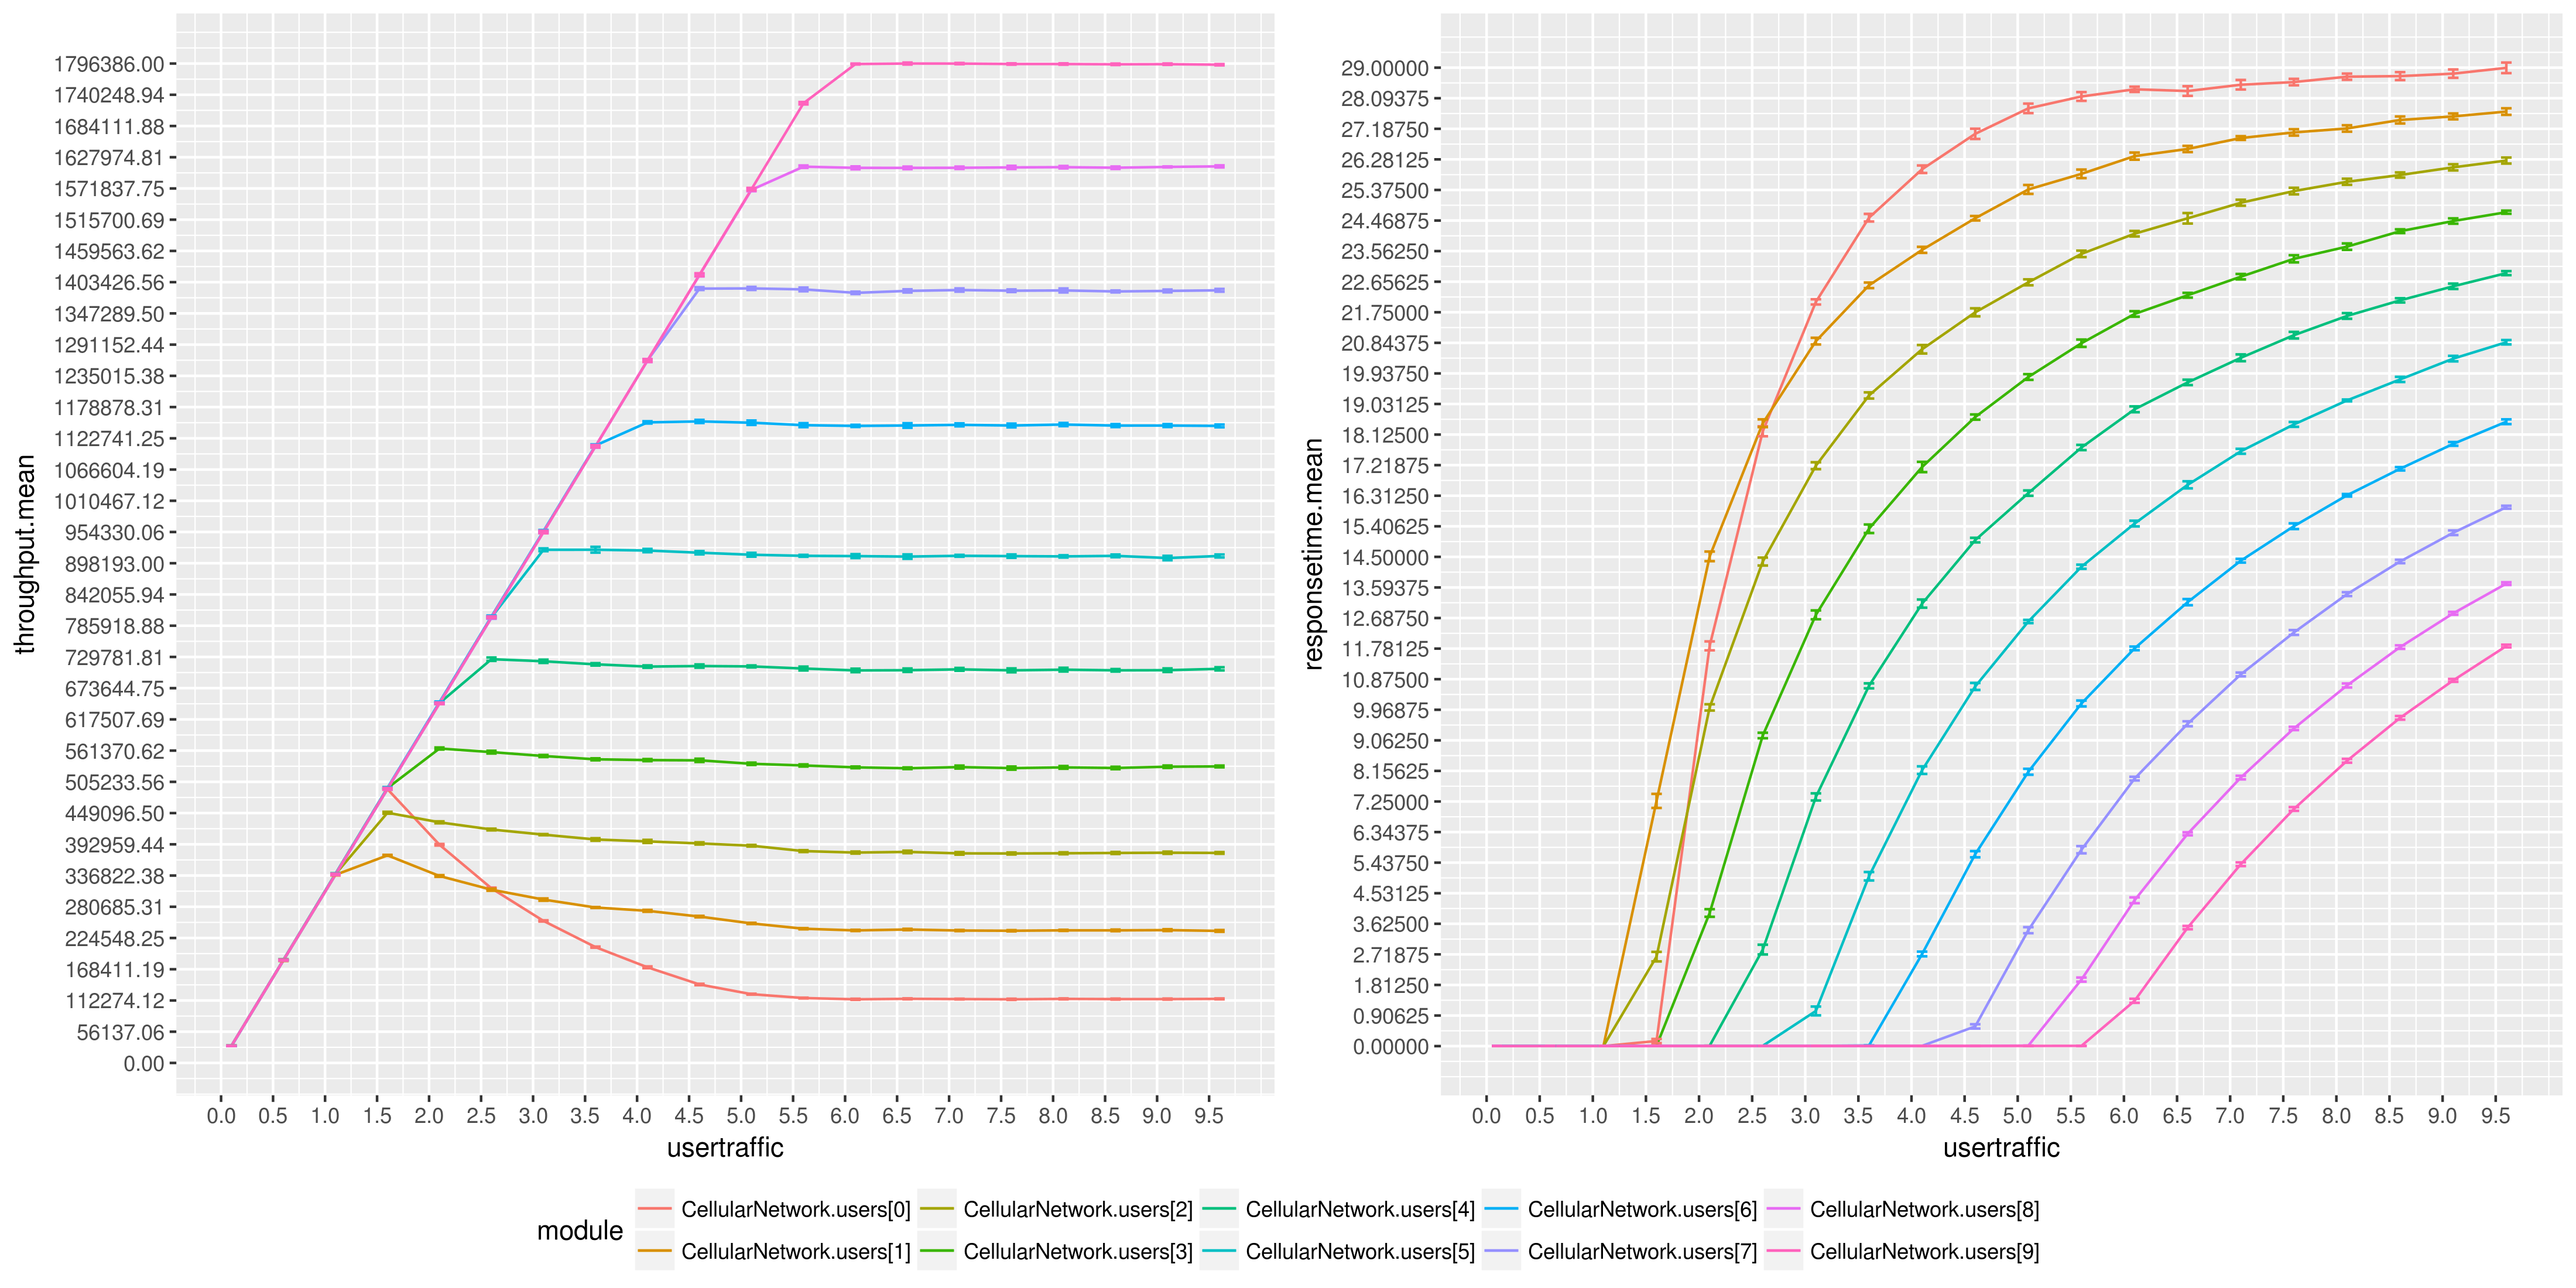
\includegraphics[width=1\textwidth]{images/binom_old}
  \caption{Binomial scenario, Modified scheduler - Simple: throughput, response time}\
  \label{fig:Binomial scenario - Simple: throughput, response time}
\end{figure}
If we consider the \texttt{user[0]} we can notice a very strange behavior. When \(0 < \lambda \leq 1.5\) it has higher throughput and smaller response time than \texttt{user[1]} and \texttt{user[2]} and this seems senseless because \texttt{user[0]} has smaller mean CQI. However this odditity can be explained by observing that, in that range of traffic, \texttt{user[9]} requires a low number of RBs but the frame must be filled and the simple rule \textbf{always} chooses the next user first which is \texttt{user[0]}. When \(\lambda\) increases, \texttt{user[9]} requires more RBs, and the throughput of \texttt{user[0]} decreases.

In this condition the distribution of throughput is absoloutely no fair since there are privileged user, the ones near the antenna, and the others that receives signal of low power so cannot achieve the same throughput.
\begin{figure}[H]
  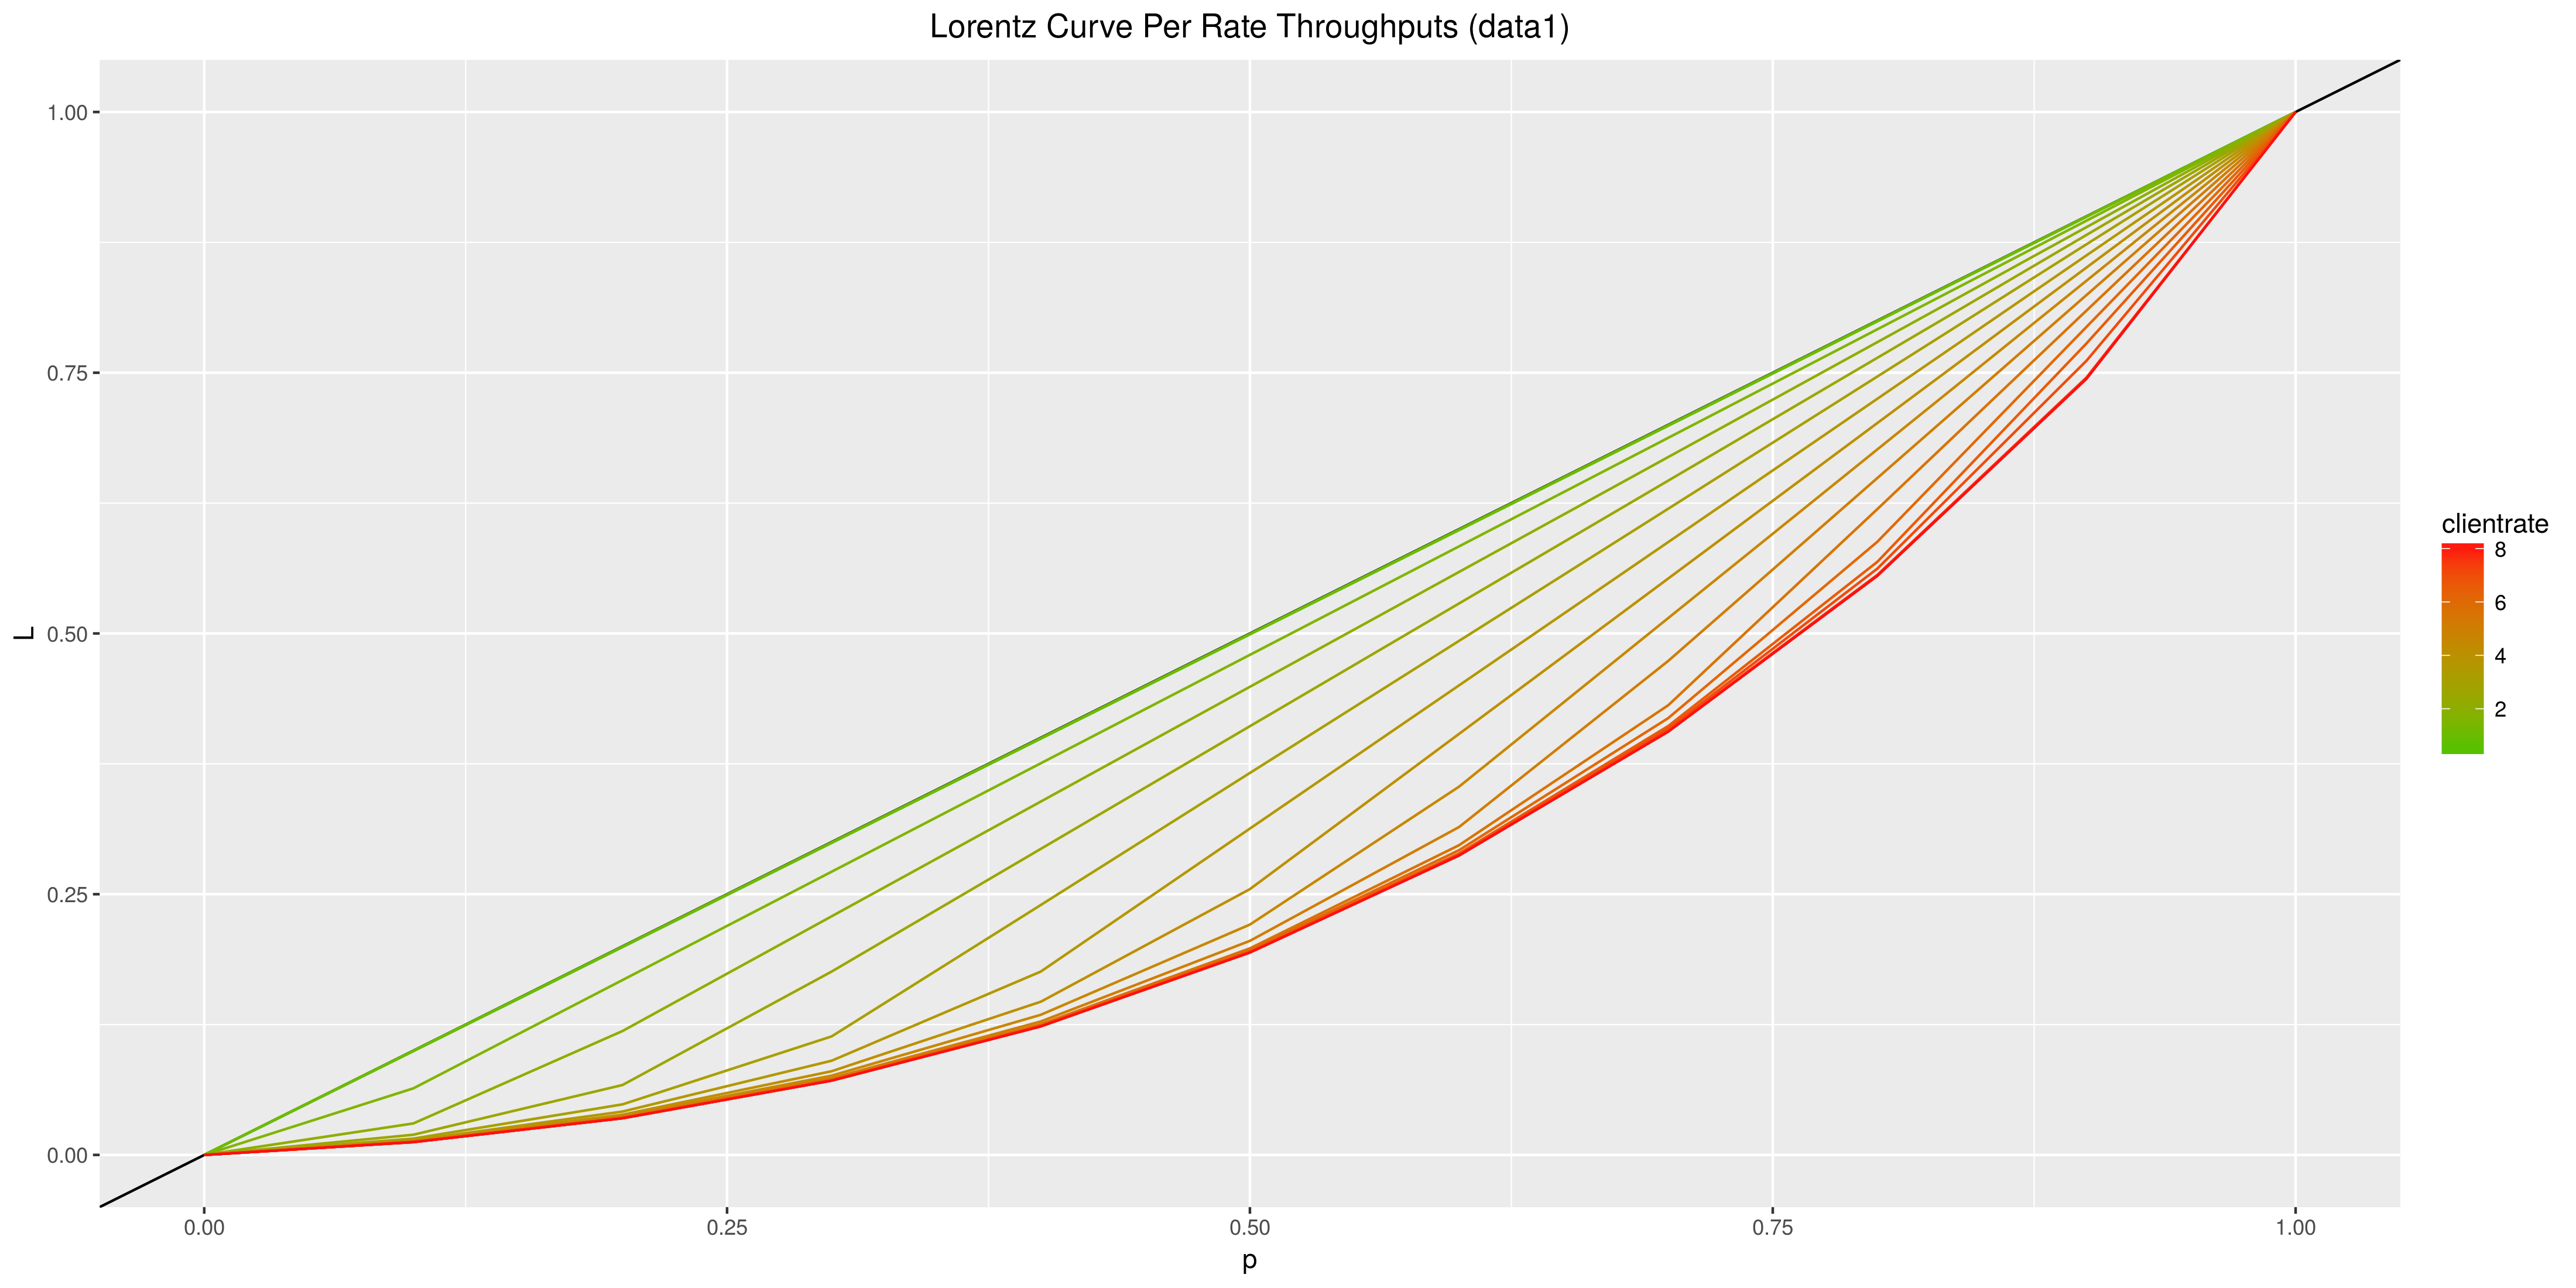
\includegraphics[width=1\textwidth]{images/lorallth-binombest.png}
  \caption{Binomial BestCQI comparison - Throughput - Lorenz Curve}
  \label{fig:lorallth-binombest}
\end{figure}

The following table shows the saturation point and the mean throghput per each user (confidence lvl 95\%).
\begin{center}
	\begin{tabular}{|c | c | c|}
	\hline
	 \textbf{user}  & \textbf{\(\lambda_{sat}\)}  & \textbf{throghput [bps]} \\ \hline
	 0 & 1.1 & $342855 \pm 1027$ \\ \hline
	 1 & 1.6 & $499558 \pm 1057$\\ \hline
	 2 & 2.1 & $652748 \pm 2600$\\ \hline
	 3 & 2.6 & $767444 \pm 3177$\\ \hline
	 4 & 3.1 & $913755 \pm 4954$\\ \hline
	 5 & 3.6 & $1093554 \pm 5318$\\ \hline
	 6 & 4.1 & $1279993 \pm 3140$\\ \hline
	 7 & 4.6 & $1434389 \pm 1780$ \\ \hline
	 8 & 5.6 & $1726384 \pm 2218$ \\ \hline
	 9 & 6.1 & $1904459 \pm 1880$ \\ \hline
	\end{tabular}
\end{center}

\section{Binomial, Best CQI Scheduler}
Now let's turn on the BestCQI policy. We are somehow expecting the same base result as the Fair scheduler, this is because \textit{frame sharing} pulls performances much less than the main filling policy (the \(currentUser\) fills up the frame until queue is empty or next packet is too big to fit). However we expect an higher throughput for higher CQI users and lower throughput for lower CQI ones w.r.t the Fair Scheduler, mainly because residual frame filling now gives priority to higher CQI.

\begin{figure}[H]
  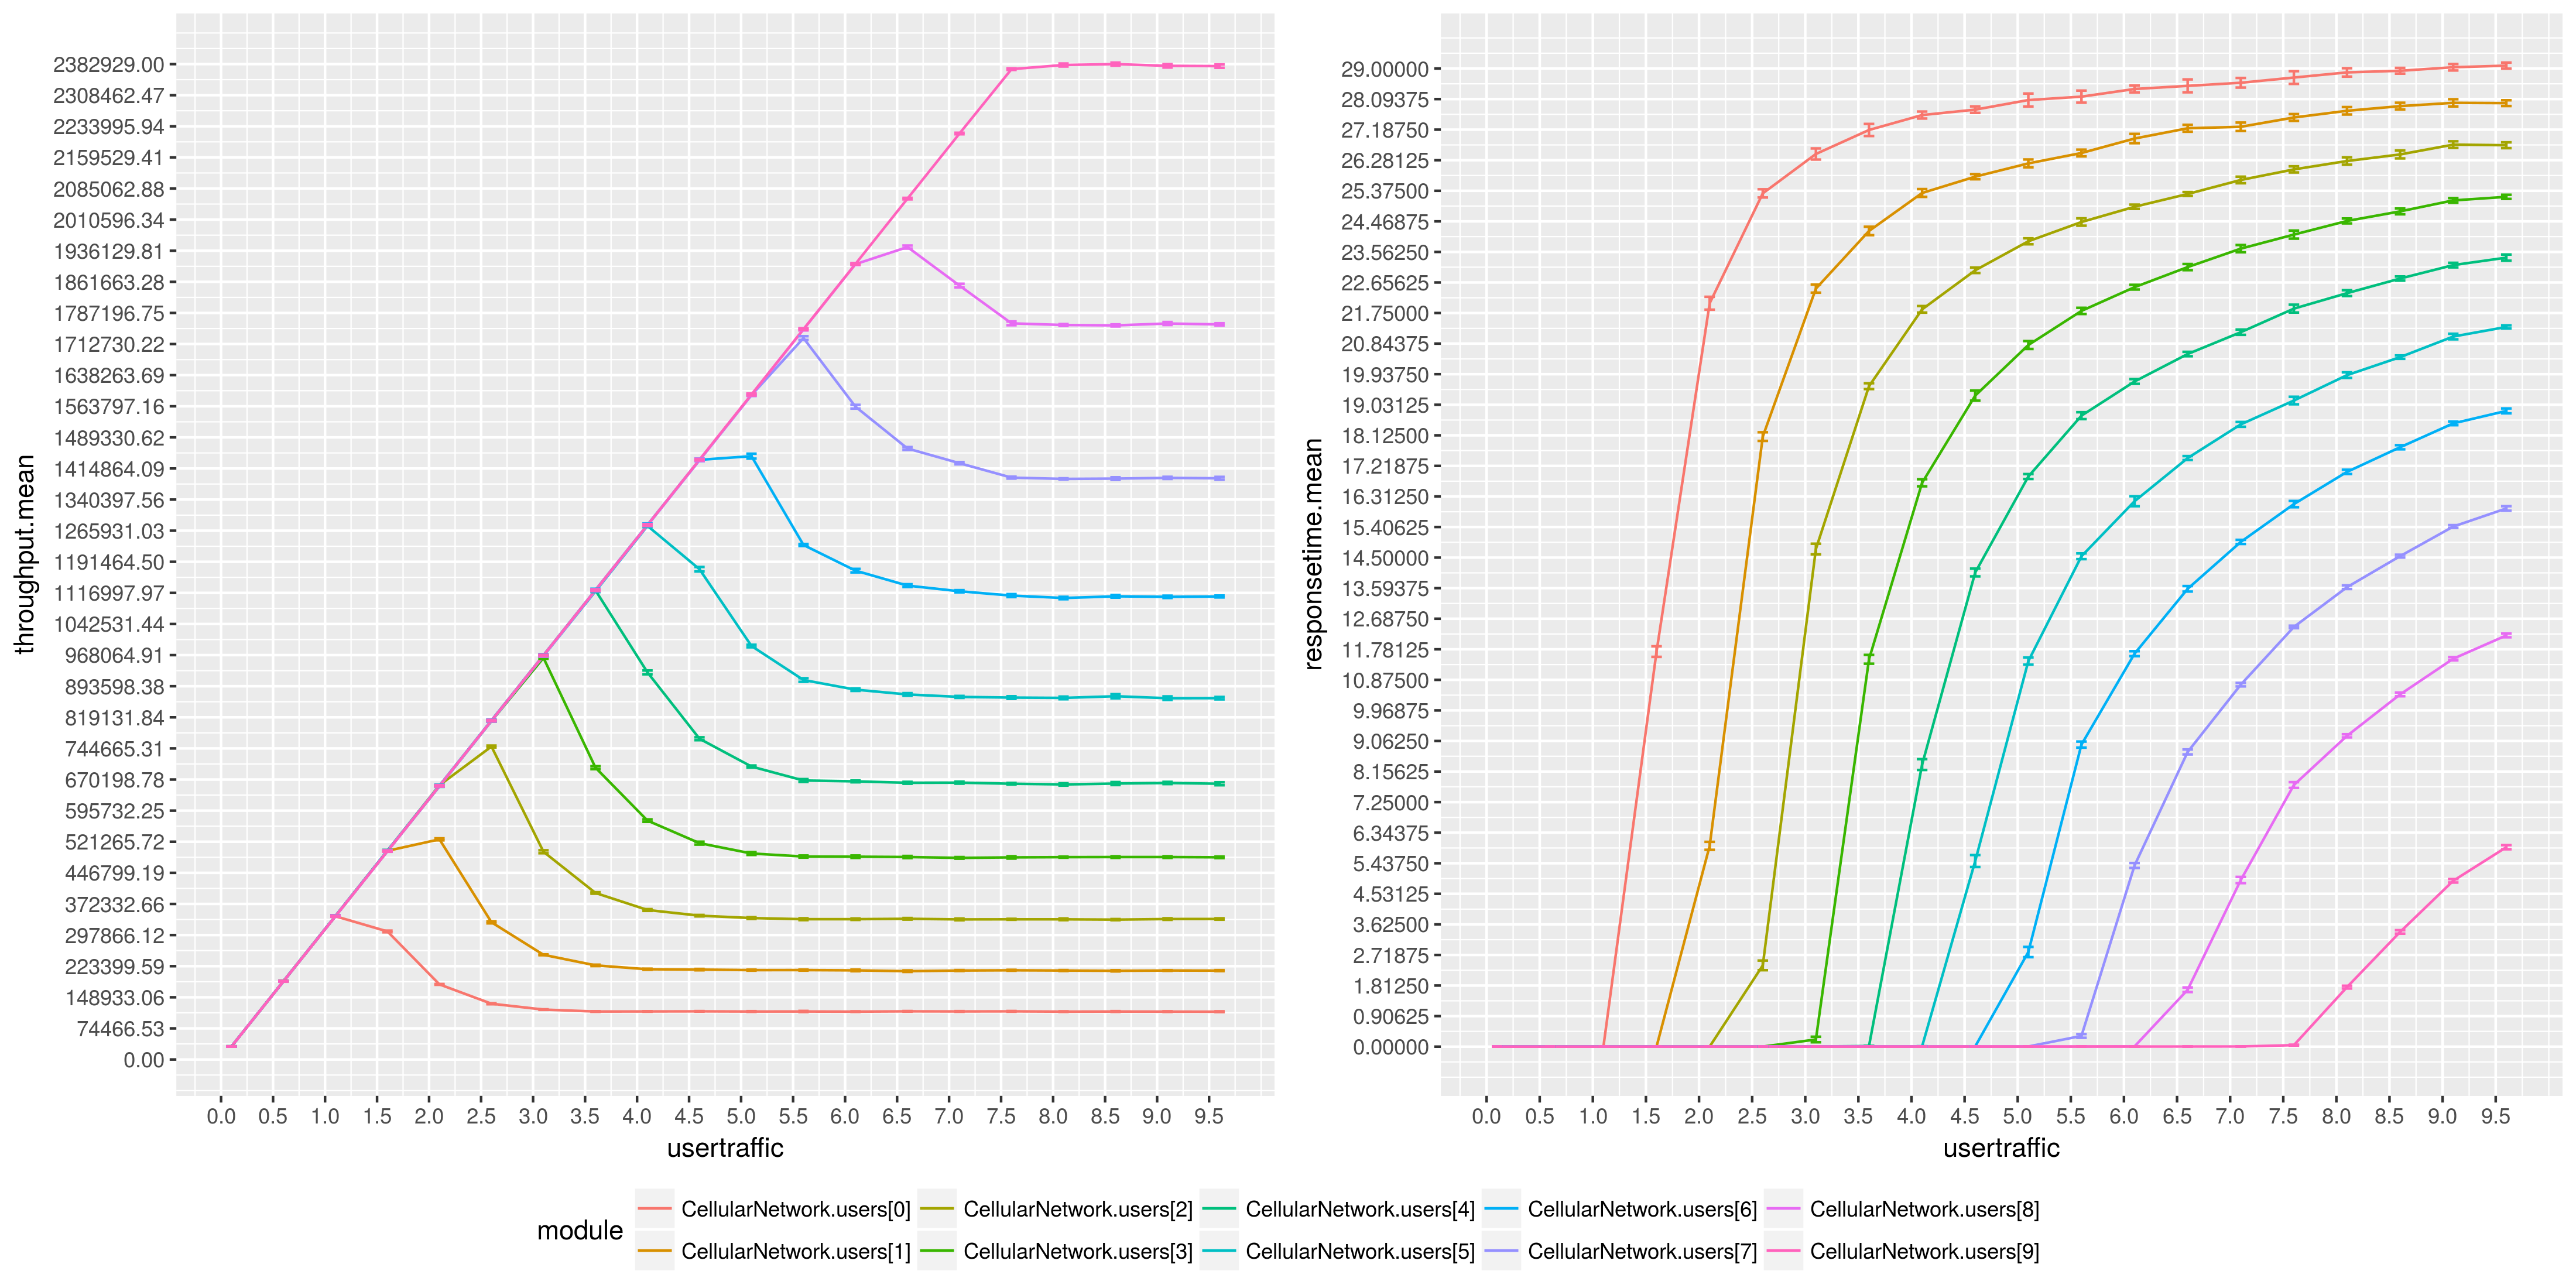
\includegraphics[width=1\textwidth]{images/all-binombest.png}
  \caption{Binomial scenario - Fair: throughput, response time}
  \label{fig:all-binombest}
\end{figure}
As we saw before, saturation points are different for each user and depend on CQI mean. However this time each throughput line has an shorter tail w.r.t. the previous experiment results, so this means that we have an higher value around the peak and lower values for higher \(\lambda\). Instead, for \texttt{user[0]} and \texttt{user[9]} there is no difference in line shapes. How can we explain this results?

As \(\lambda\) gets higher, each user come to its saturation point: the first is \texttt{user[0]} which will use some RBs from the other users before reaching the peak, just as we saw in the last chapter. The next user to get to saturation point is \texttt{user[1]}, which will start to reclaim the residual frame and, eventually, start to use RBs from other users. This is also what we saw before, but there is an important difference: \texttt{user[1]} has priority over \texttt{user[0]} when doing the residual frame filling, because it has an higher CQI. This means that \texttt{user[1]} will eventually take \textit{all} the residual RBs for himself at some point, leaving \texttt{user[0]} without extra RBs. In the same way, when \texttt{user[2]} start to reclaim its RBs and then the other users residual frames, it basically takes all extra RBs also from \texttt{user[1]}, and we can continue until \texttt{user[9]}, which, at the end, takes all!
We basically explained:
\begin{itemize}
	\item The higher peak, due to the higher number of reclaimed extra RBs (from other users residual frames)
	\item The shorter tail, which is caused by having less RBs when higher CQI users reclaim all the extra RBs
	\item The unchanged shape of \texttt{user[0]} and \texttt{user[9]}, the first because it is the first to reclaim residual frames from the other users, and the second because it is the higher CQI and reclaims all at the end (highier value of \(\lambda\))
\end{itemize}

If we want to compare shapes, let's take, for example, \texttt{user[5]} and compare in both experiments, plotting them:

\begin{figure}[H]
  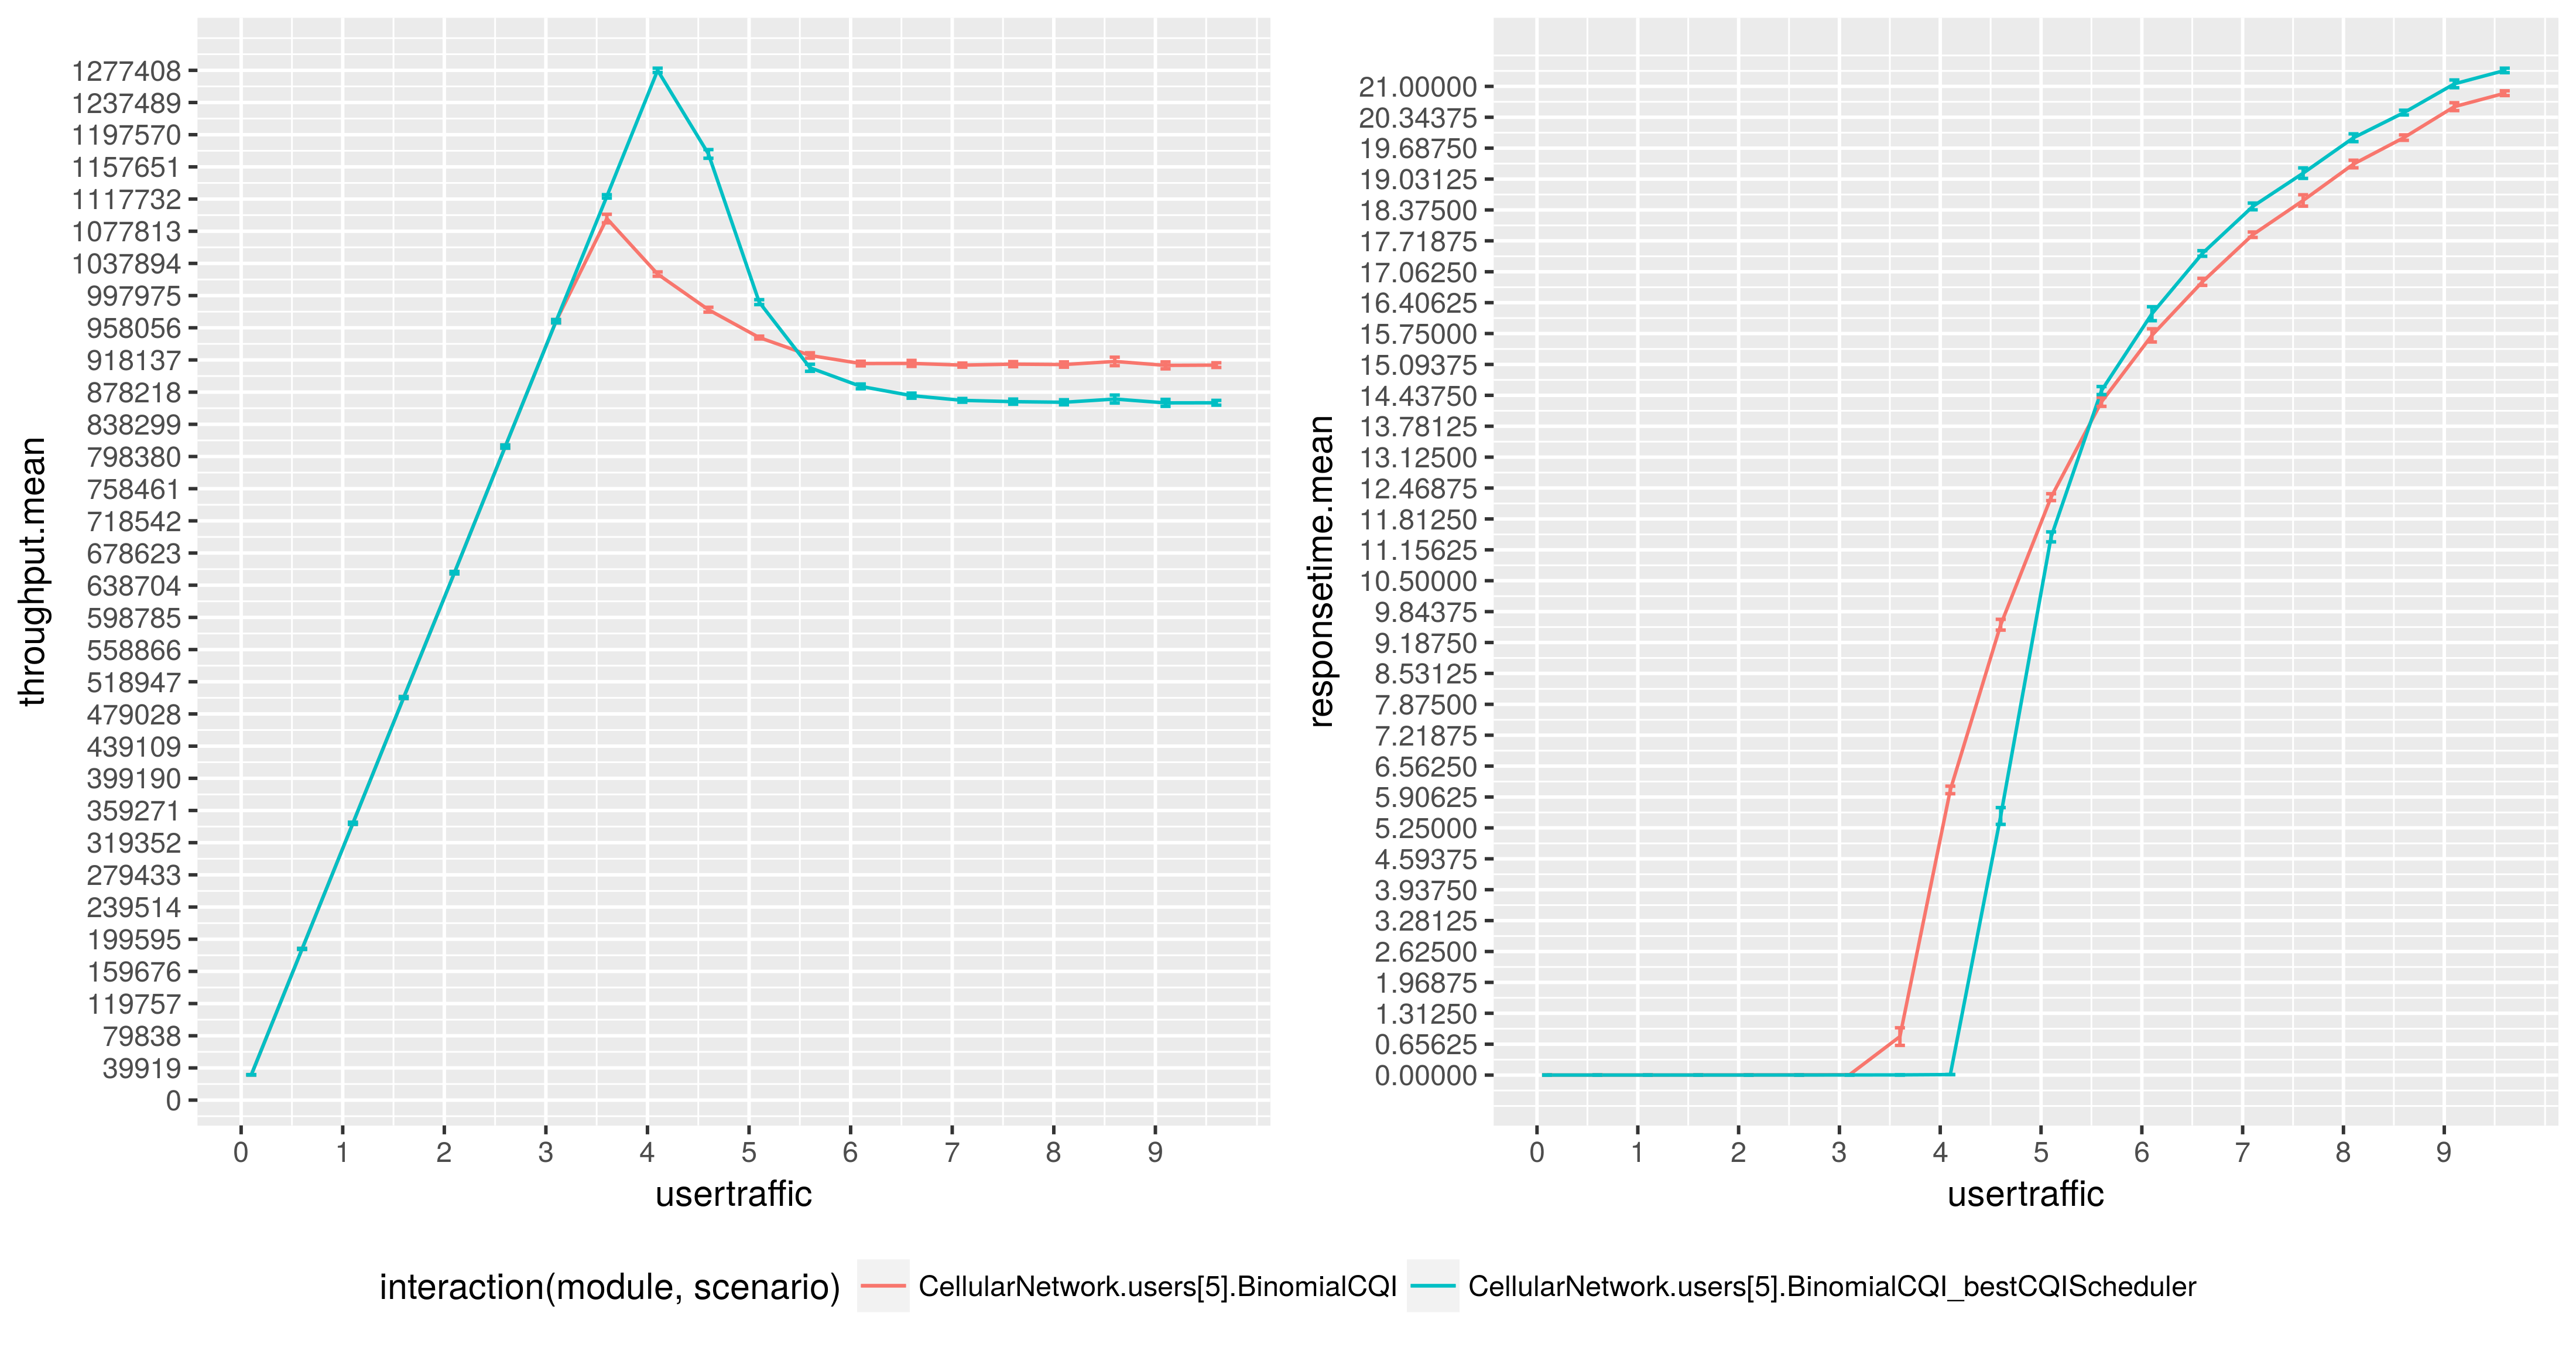
\includegraphics[width=1\textwidth]{images/th-binom-binombest-5-5.png}
  \caption{Binomial Fair/Binomial BestCQI comparison - throughput, response time}
  \label{fig:th-binom-binombest-5-5}
\end{figure}

Let's check how simulated resource blocks are distributed among users at rate \(\lambda = 4.1\) (around \texttt{user[5]} throughput peak), comparing the two experiments:

\begin{figure}[H]
  \includegraphics[width=1\textwidth]{images/{allrbbars-binom-binombest-4.1}.png}
  \caption{Binomial Fair/Binomial BestCQI comparison - Resource Block count}
  \label{fig:allrbbars-binom-binombest-4.1}
\end{figure}

\texttt{user[5]} basically reclaimed all the missing RBs of lower CQI users, while instead they are fairly distributed among users when using the Fair CQI policy.

RB distribution unfairness can be confirmed also using a Lorenz Curve graph:
\begin{figure}[H]
  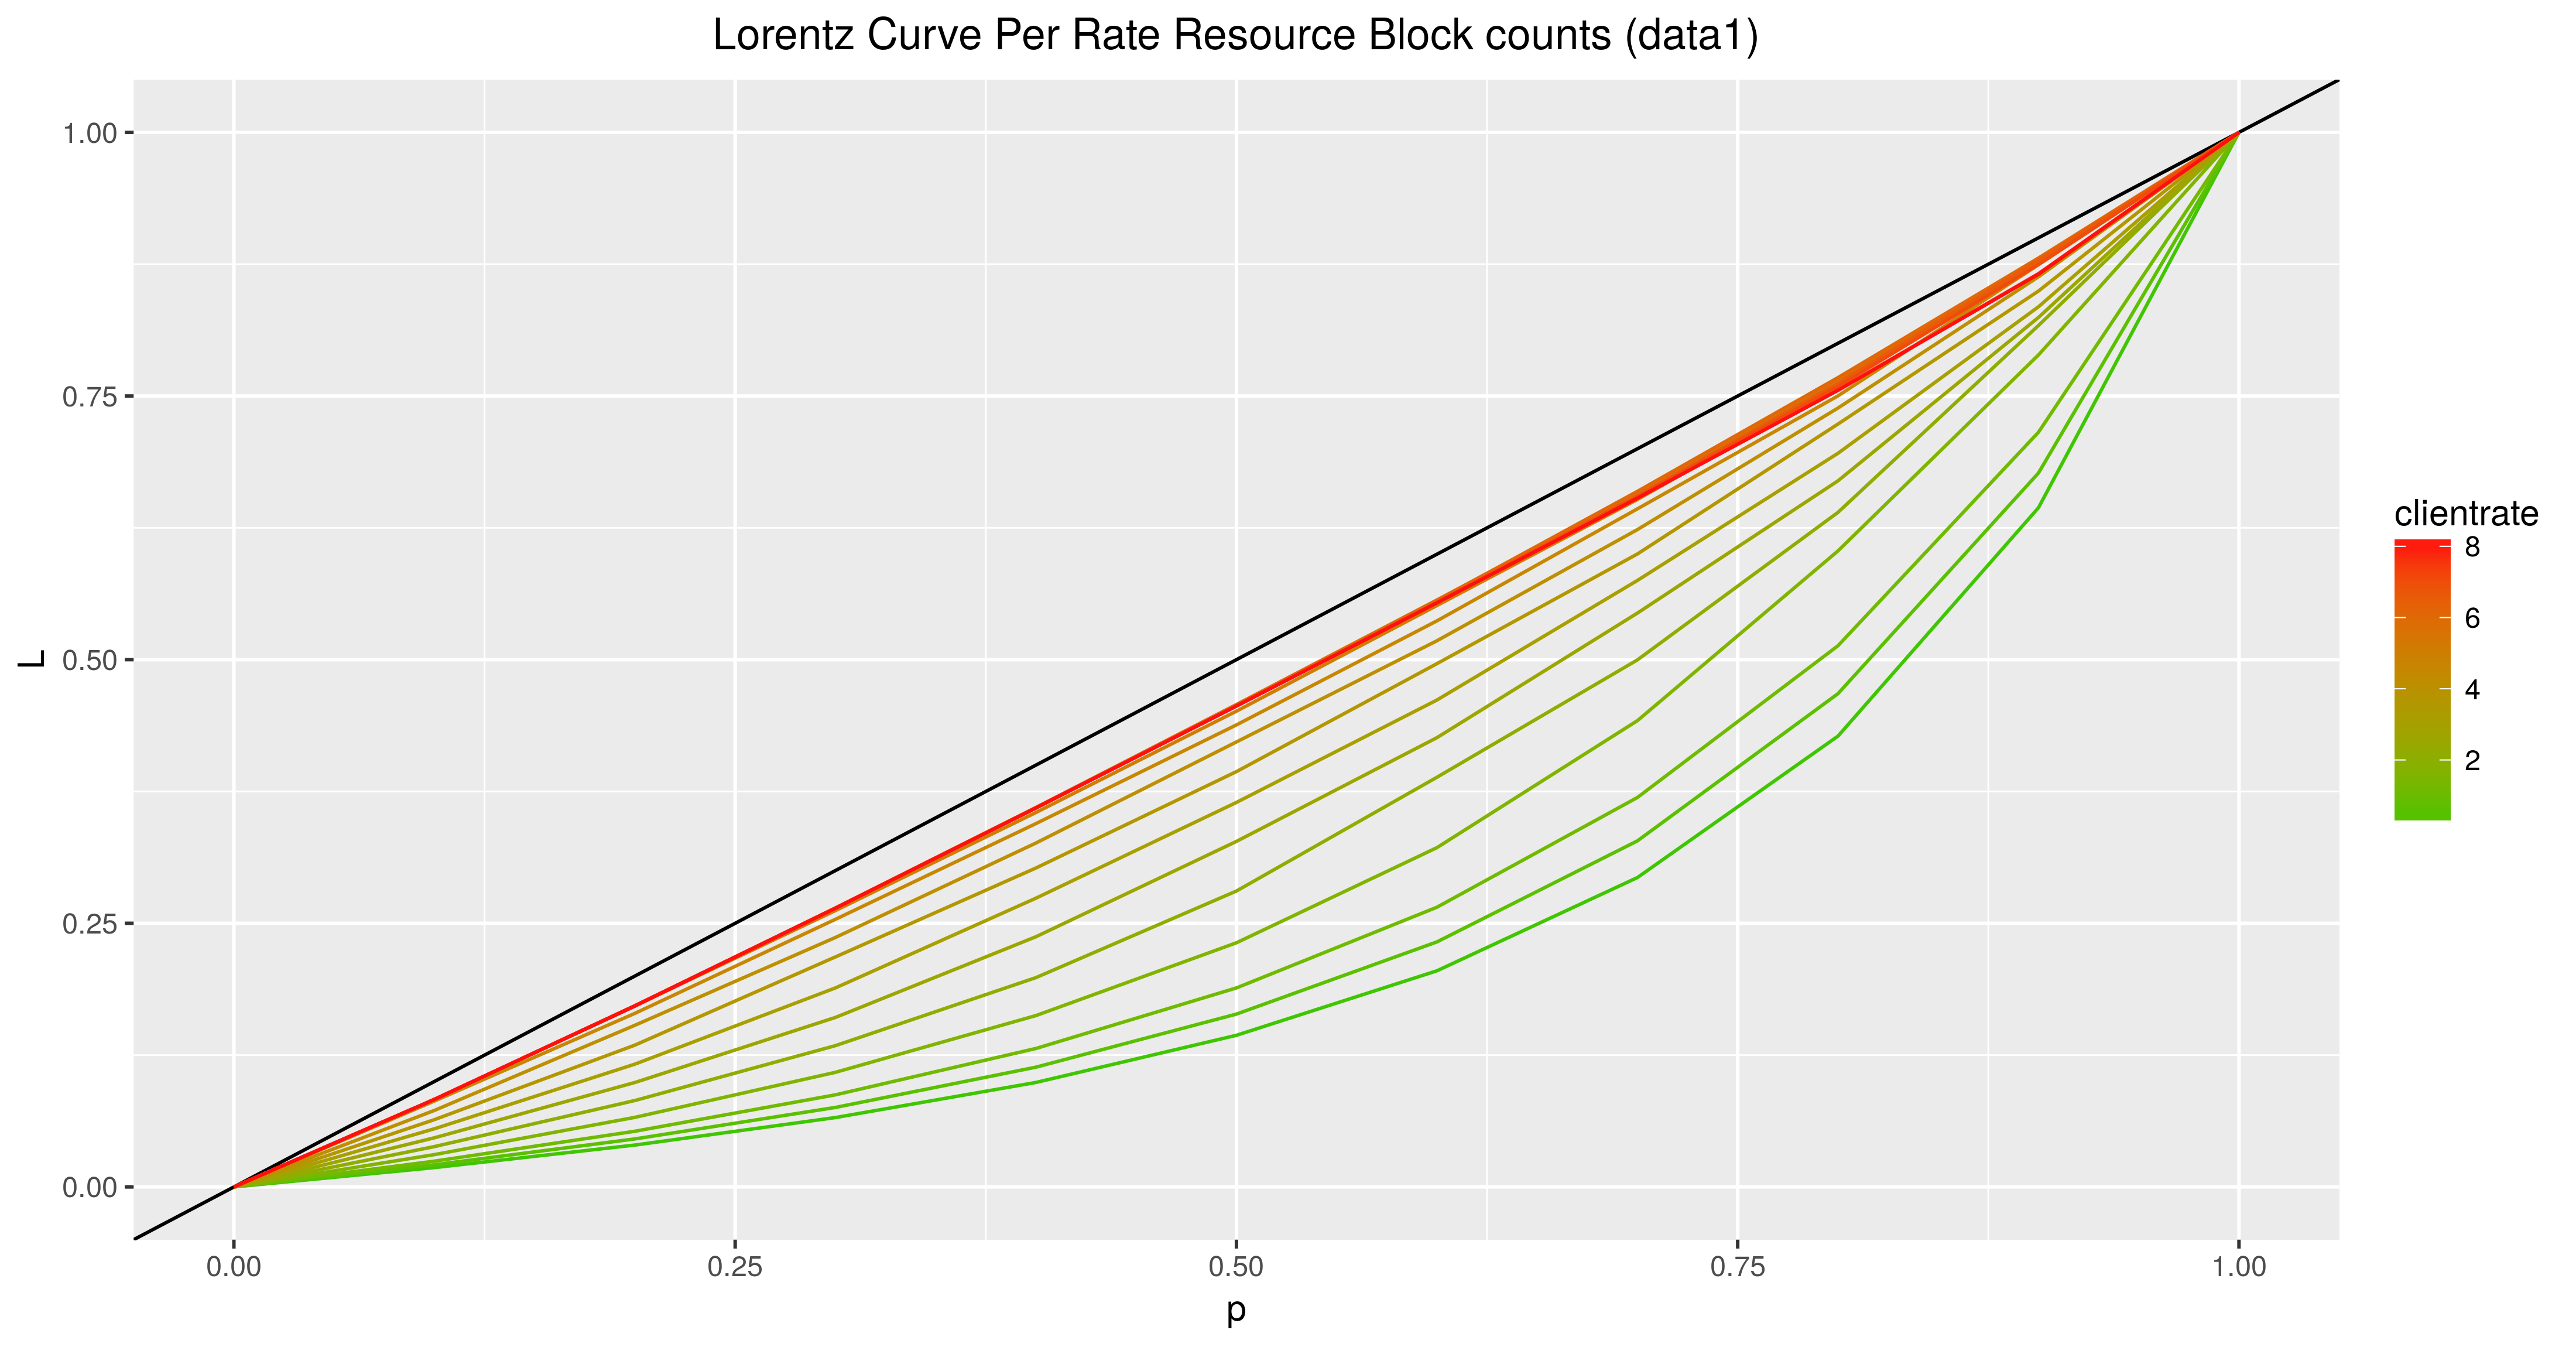
\includegraphics[width=1\textwidth]{images/lorallrb-binombest.png}
  \caption{Binomial BestCQI comparison - Resource Block - Lorenz Curve}
  \label{fig:lorallrb-binombest}
\end{figure}
The graph in \ref{fig:lorallrb-binombest} shows curves for each value of \(\lambda\). We can see that fairness is higher at the end just because \texttt{user[9]} takes all the extra RBs and leaves the other users with nothing that their own RBs, which are of the same count for all (25). On the other hand Fairness is higher when \(\lambda\) is low because first users takes all the extra RBs from the higher CQI users, and the higher CQI users use less RBs due to the very low interarrival rate.

Throughput unfairness can also be shown using a Lorenz Curve graph:
\begin{figure}[H]
  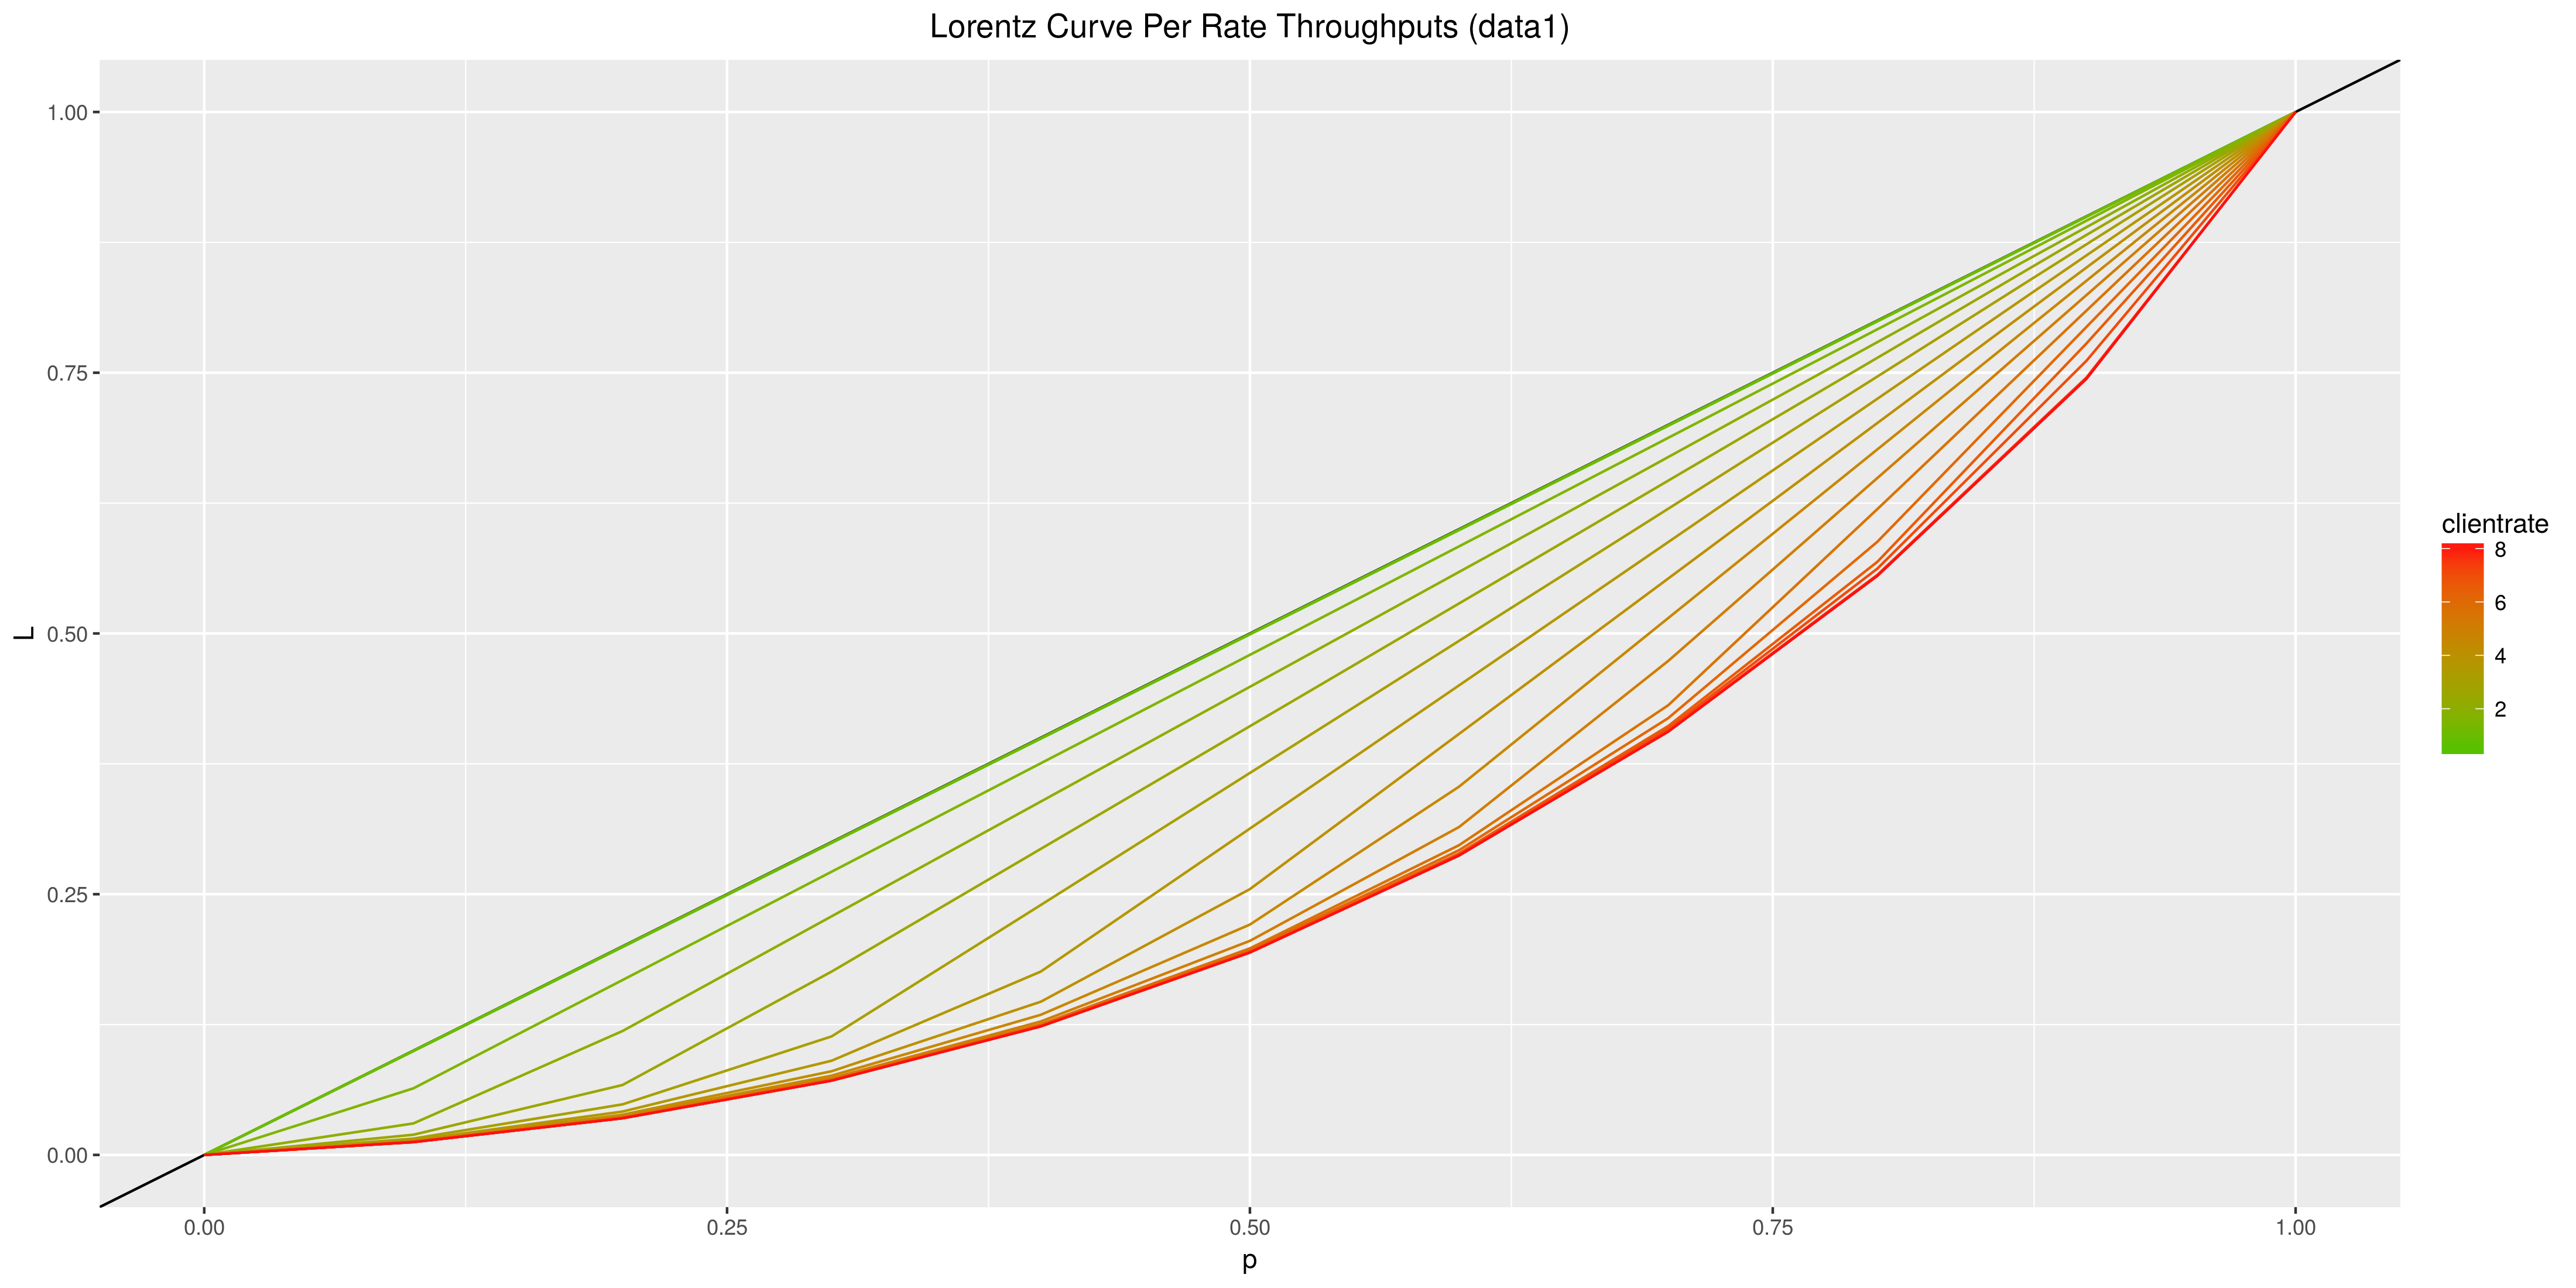
\includegraphics[width=1\textwidth]{images/lorallth-binombest.png}
  \caption{Binomial BestCQI comparison - Throughput - Lorenz Curve}
  \label{fig:lorallth-binombest}
\end{figure}

In this case we must consider that this measure heavly depends on the CQI distribution: the higher unfairness is shown when \(\lambda\) is high, because \texttt{user[9]} uses all extra RBs, and the lower unfairness is shown for low \(\lambda\) values, where no one has yet reached saturation.

Now let's take a zoom to the plot of response time. If we compare the following graph with the Binomial Fair one, we note that saturation points are shifted to right. 
\begin{figure}[H]
  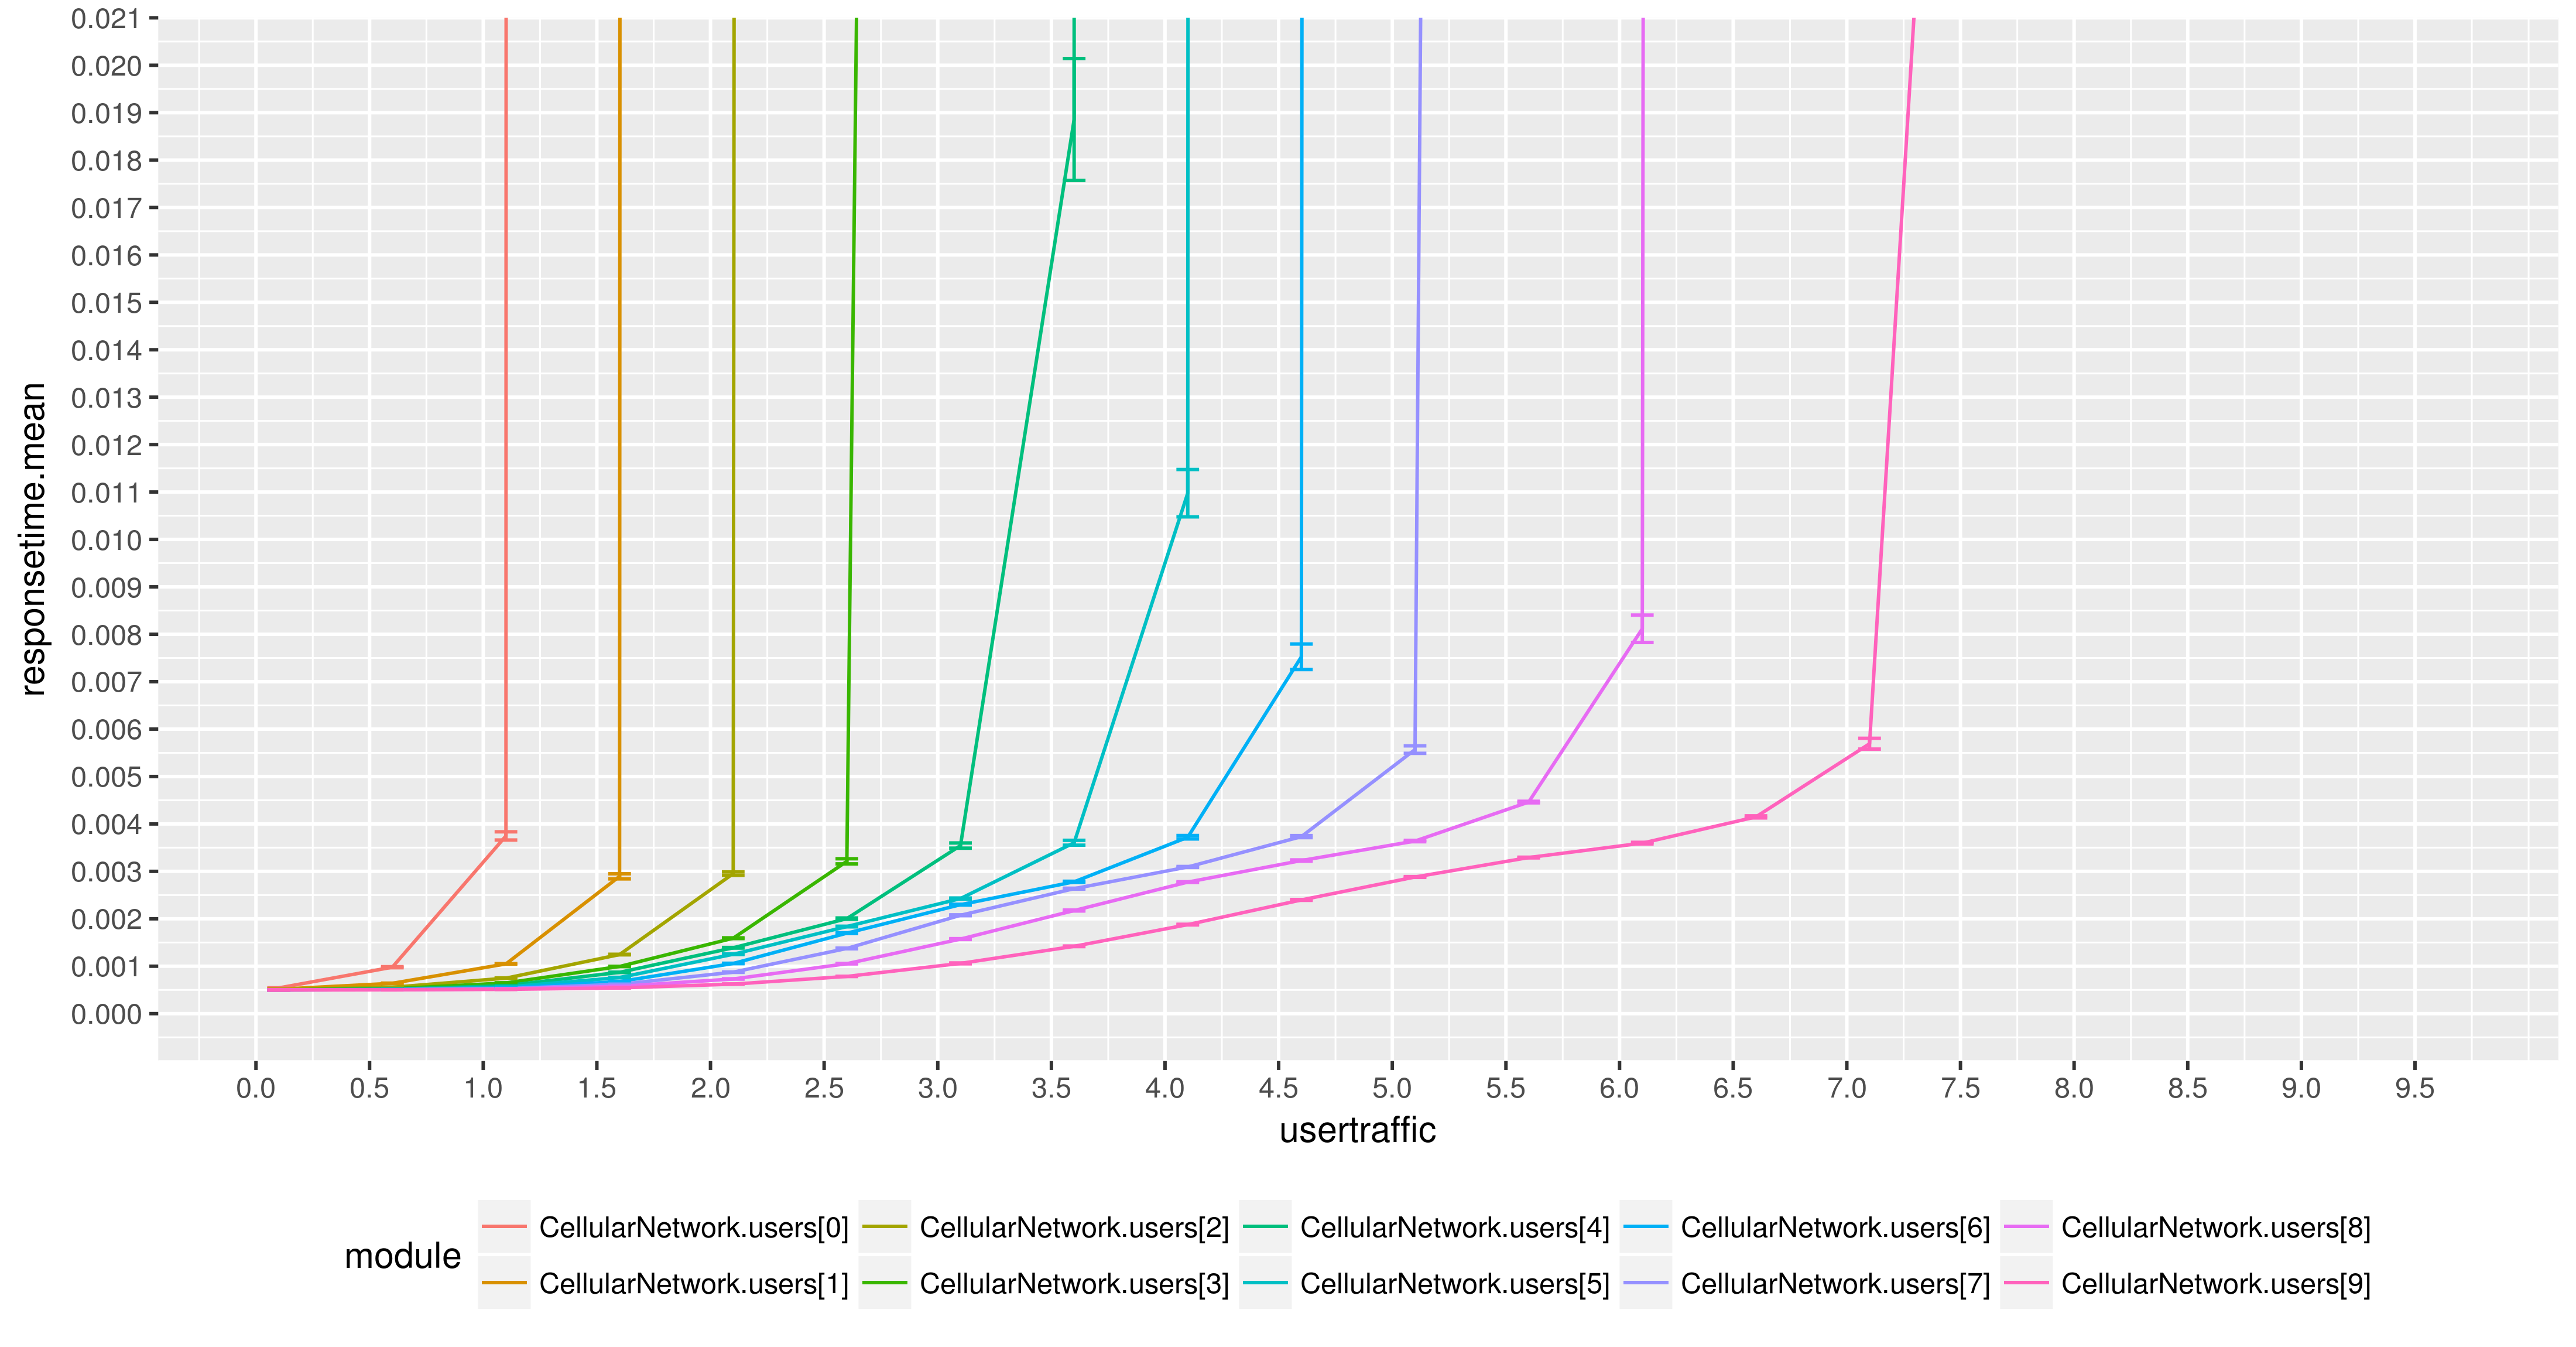
\includegraphics[width=1\textwidth]{images/allrt-binombest.png}
  \caption{Binomial scenario - BestCQI: response time zoom}
  \label{fig:allrt-binombest}
\end{figure}
As explained before this is due the extra RBs that users with higher mean CQI can use for the frame filling. The most noticeable change is for \texttt{user[9]}. In the Binomial Fair scenario its response time has a spike around \(\lambda = 6.1\), now it is bounded and well defined until \(\lambda = 7.1\)

In the following table there is a summary of throughput in \(\lambda_{sat}\) per each user.
\begin{center}
	\begin{tabular}{|c | c | c|}
	\hline
	 \textbf{user}  & \textbf{\(\lambda_{sat}\)}  & \textbf{throghput [bps]} \\ \hline
	 0 & 1.1 & $342852 \pm 1028$ \\ \hline
	 1 & 1.6 & $499580 \pm 1092$\\ \hline
	 2 & 2.6 & $749257 \pm 2282$\\ \hline
	 3 & 3.1 & $961496 \pm 2240$\\ \hline
	 4 & 3.6 & $1123105 \pm 1315$\\ \hline
	 5 & 4.1 & $1277408 \pm 2667$ \\ \hline
	 6 & 4.6 & $1435511 \pm 2868$\\ \hline
	 7 & 5.6 & $1727047 \pm 4506$ \\ \hline
	 8 & 6.1 & $1904025 \pm 2349$ \\ \hline
	 9 & 7.6 & $2370866 \pm 1914$ \\ \hline
	\end{tabular}
\end{center}


Let's now compute the antenna total throughput:
\begin{figure}[H]
  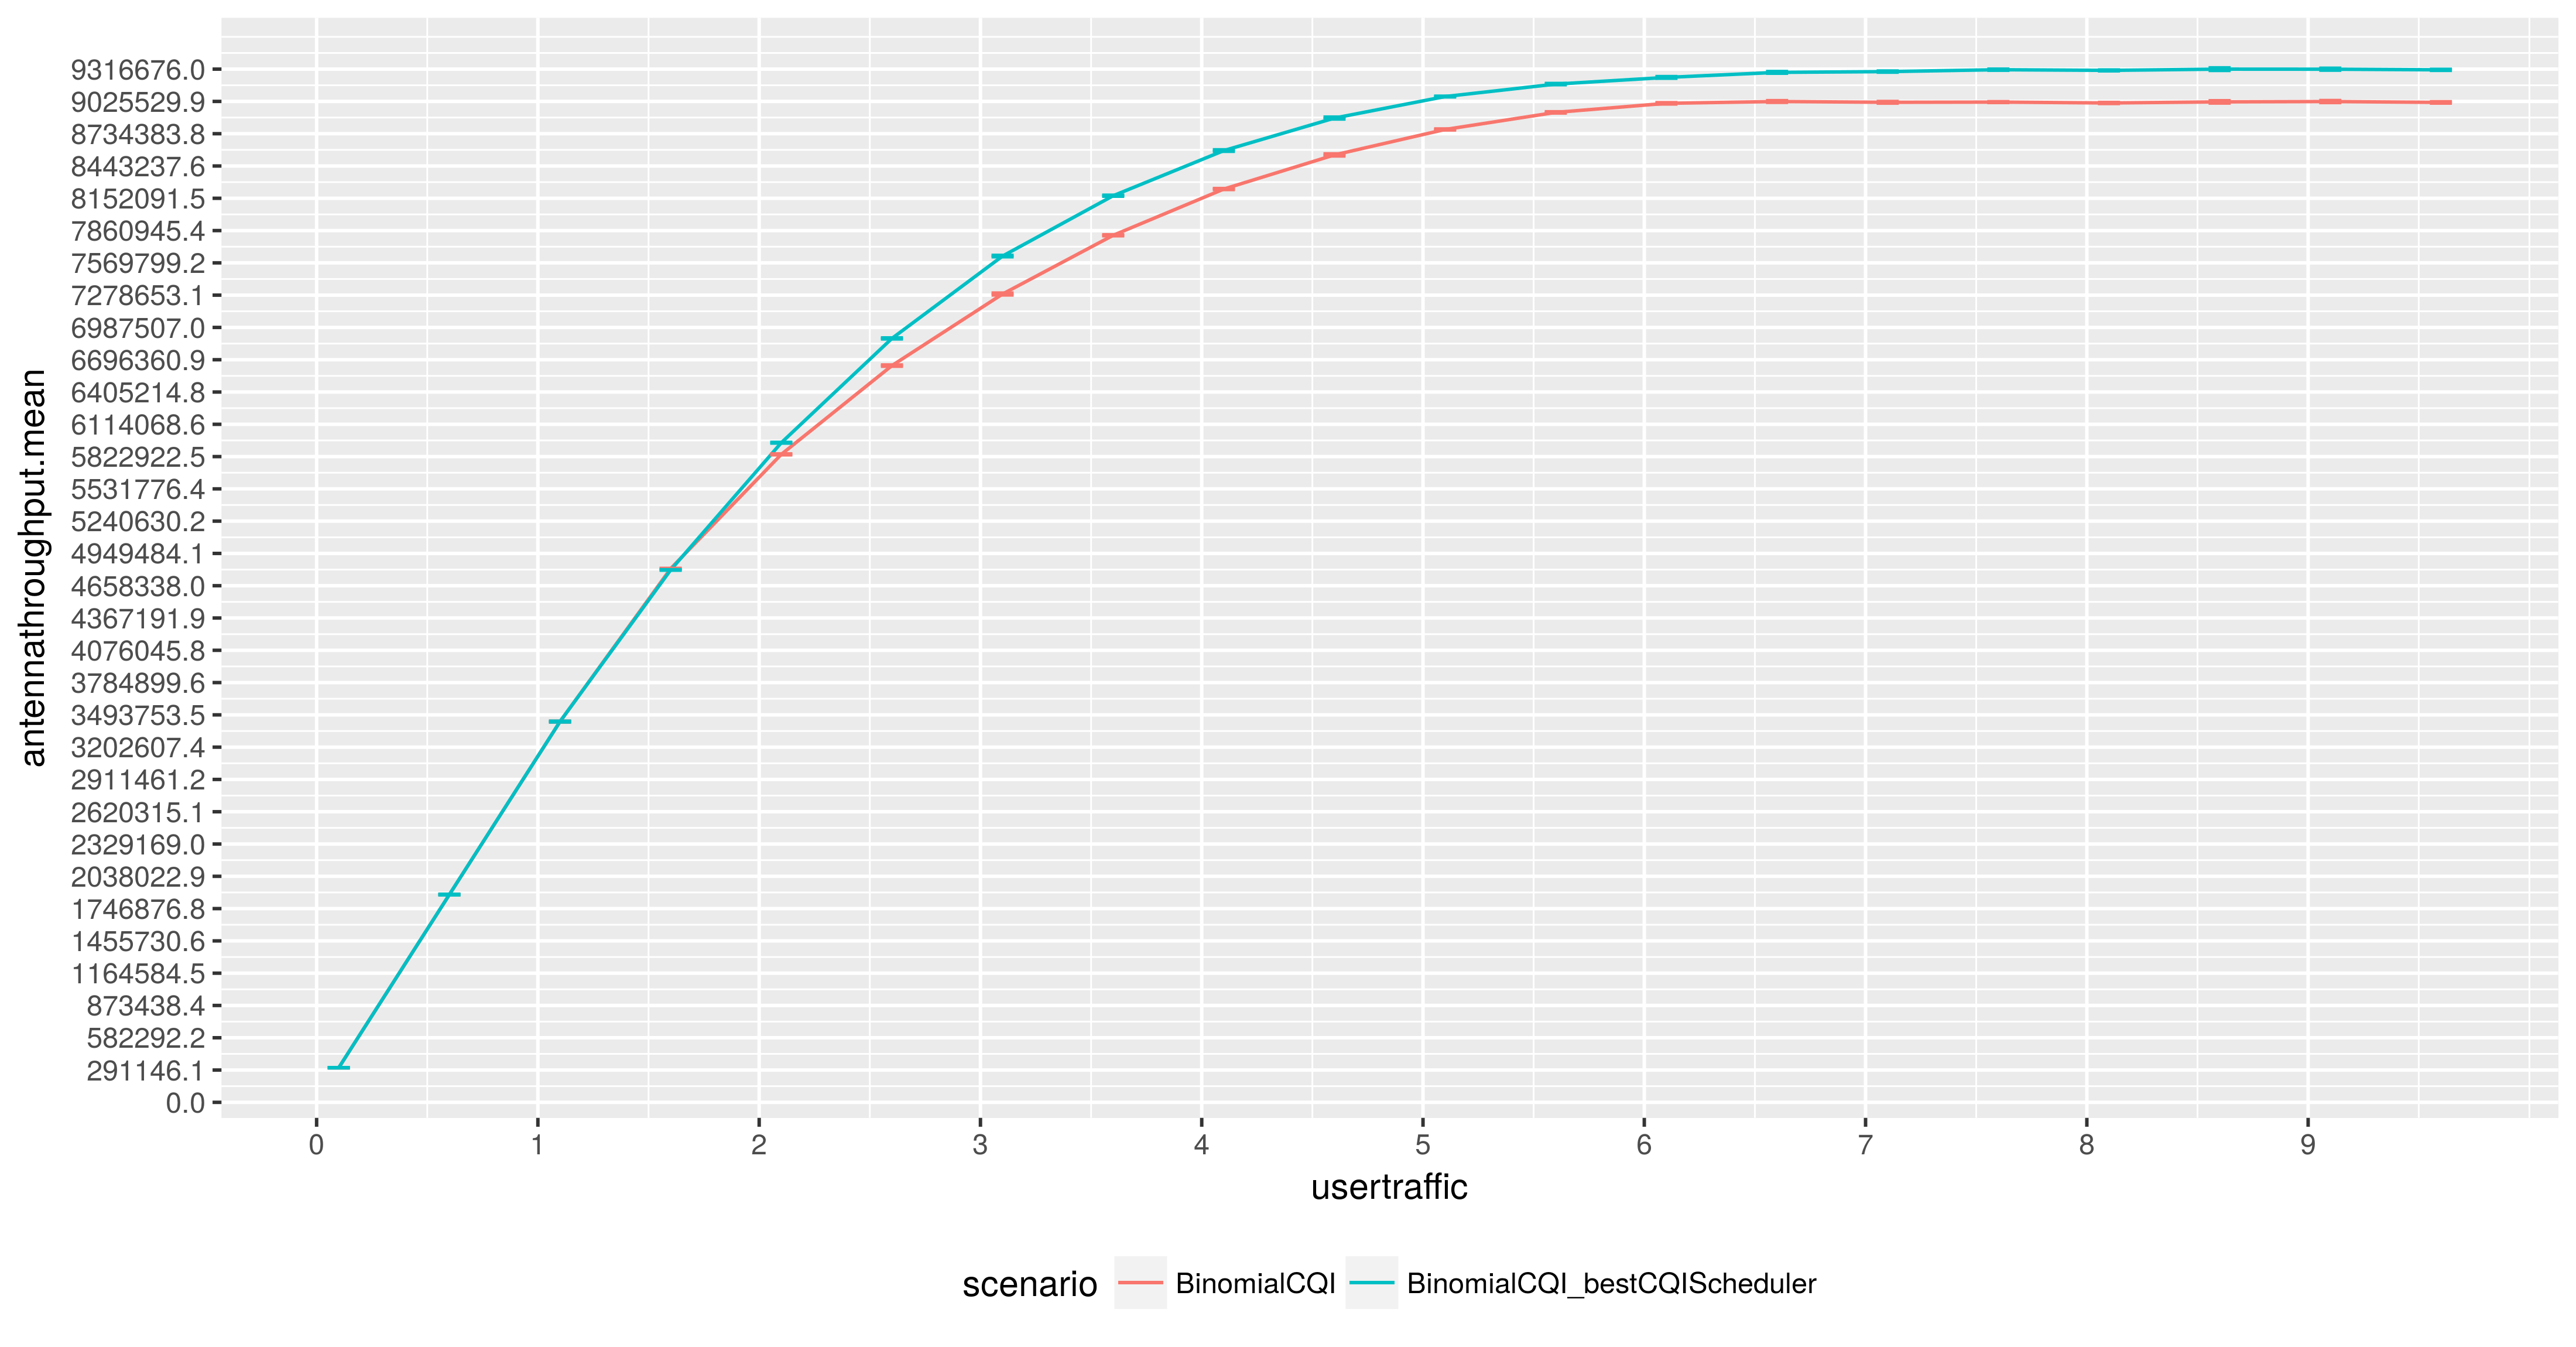
\includegraphics[width=1\textwidth]{images/thantenna-2.png}
  \caption{Binomial Fair/Binomial BestCQI comparison - Total Antenna Throughput}
  \label{fig:thantenna-2}
\end{figure}

Binomial BestCQI seems the best choice to maximize this throughput. We must note that the BestCQI algorithm basically reallocates residual frame RBs to the users with the best CQI, but the total number of RBs remains the same: however better CQI correspond to higher RB sizes, which will increase the total antenna throughput.

So, is Best CQI policy scheduler the better choice for Binomial CQIs scenarios? It depends. As we saw, giving priority to users with higher CQI leads to a decreased unfairness. However channel usage efficiency will go up as the throughput for users with higher CQI, but the gained throughput will be shared only among higher CQI users. Response time just follows the throughput trend.